\documentclass[12pt]{book}
\usepackage[utf8]{inputenc}
\usepackage{amsmath, amssymb, amsfonts, amsthm}
\usepackage{bbm}
\usepackage{url}
\usepackage{geometry}
 \geometry{
 a4paper,
 left=20mm,
 right=20mm
 }
\linespread{1.1}

\usepackage{pgfplots}
\pgfplotsset{compat=newest}
\usepackage{subfigure}

\usepackage{mathtools}
\mathtoolsset{showonlyrefs}

\usepackage{xcolor}
\definecolor{linkcolour}{rgb}{0,0.2,0.6}

\usepackage{hyperref}
\hypersetup{colorlinks,breaklinks,urlcolor=linkcolour, linkcolor=linkcolour}

\renewcommand{\iff}{\Leftrightarrow}

\newtheorem{theorem}{Theorem}[chapter]
\newtheorem{prop}[theorem]{Proposition}
\newtheorem{cor}[theorem]{Corollary}
\newtheorem{lemma}[theorem]{Lemma}

\theoremstyle{definition}
\newtheorem{defn}{Definition}[chapter]

\theoremstyle{remark}
\newtheorem{ex}{Example}[chapter]
\newtheorem{rmk}[theorem]{Remark}

\usepackage{enumitem}
\setenumerate[1]{label=(\roman*)}

\title{Applied Stochastic Processes Notes}
\author{Trevor Winstral}
\date{Spring Semester 2021}
\setcounter{chapter}{-1}

\begin{document}
\maketitle
\tableofcontents 
\newpage

\chapter{Introduction}
\textbf{Mathematical Definition of Stochastic Processes} We want to describe a process evolving in time. The most relevant for us will be: Discrete time ($I=\mathbb{N}$) and Continuous time ($I=\mathbb{R}$).

\begin{defn}
	Let $(E, \xi)$ be a measurable space. A discrete stochastic process with state space $E$ is a collection $X=(X_n)_{n \in \mathbb{N}}$ of RVs with values in $E$.
\end{defn}

\begin{defn}
A continuous stochastic process is a collection $(X_t)_{t \in \mathbb{R}_+}$ of RVs with values in $E$.
\end{defn}

In this class we will work with jump processes, ie when $E$ is finite or countable.
We will work with:
\begin{enumerate}
	\item Discrete time Markov Chains $I=\mathbb{N}$ and $E$ finite or countable
	\item Poisson renewal processes $I=\mathbb{R}_{+}$ and $E= \mathbb{N} $
	\item Continuous Markov Chains $I= \mathbb{R}_{+}$ and $E$ finite or countable
\end{enumerate}
We will not work with Brownian Motion.

\begin{ex}[Simple Random Walk] 
	State Space $\mathbb{Z}^{d}$, $x,y$ are neighbors $\iff \|x-y\|_{1}=1$. An electron is starting at 0, and each step it jumps uniformly to one of the neighbors. How should we define this?

\end{ex}

\begin{defn}[SRW]
	Let $(Z_n)_{n \in \mathbb{N}}$ iid, $\mathbb{P} \left[ Z_n = \pm e_i \right] = \frac{1}{2d}$ where $e_i$ is 1 in the i'th slot. $X_n := \sum_{k=1}^n Z_n= X_n + Z_{n+1}, X_0=1$. $\forall m,n X_m$ and $X_n$ are dependent.  The $X_n$ do satisfy the Markov property: Conditional on $X_n=x$ then $(X_{m+n})_{n \geq 0}$ is a SRW starting at $x$ independent of $(X_1,...,X_m)$.
\end{defn}

Will the SRW return to 0?
\begin{theorem}[Polya]\ \\ \indent
	If $d=1,2$ then $\mathbb{P} \left[ (X_n) \text{ visits x infinitely many times} \right] =1$ \\ \indent
	If $d\geq3$ then $\mathbb{P} \left[ (X_n) \text{ visits x only finitely many times} \right] =1$
\end{theorem}

\begin{ex}[Poisson Process]
	We want to define and study $N_t$ the number of cars passing a point during $[0,t]$.
\end{ex}

\begin{defn}
	$T_1 =$ passage of time of the first car, $T_2=$ time between car 1 and car 2, etc. 
\begin{itemize}
	\item $(T_i)$ are iid
	\item $(T_i)$ are memoryless:  $\mathbb{P} \left[ T_1 \geq t+s | T_1 \geq s \right] = \mathbb{P} \left[ T_1 \geq t \right] $ 
	\item Regularity: $\mathbb{P} \left[ T_1 \geq s \right] $ is 'nice'
\end{itemize}
This implies that $\mathbb{P} \left[ T_1 \geq s \right] = e^{- \lambda s}, \quad \lambda>0$
\end{defn}

Let $(T_i)_{i\geq1}$ iid $exp(\lambda)$ RV. $N_t = \sum_{i\geq1}\chi_{T_1 + ... + T_i \leq t}$ \newline
Dependencies:
\begin{itemize}
	\item $N_{t+s}-N_t \sim Pois(\lambda s)$
	\item Markov Property
\end{itemize}
LLN: $ \frac{N_t}{t} \to_{t \to \infty} \frac{1}{\lambda}$





\newpage

\chapter{Markov Chains and Generalities}

\textbf{Framework}: $(\Omega, \mathcal{F}, \mathbb{P})$ Probability Space, $E$ finite or countable set with the $\sigma$-algebra $2^E$

\noindent
\textbf{Outset} We would like to define a class of processes such that the evolution of the process is memoryless, but still location dependent. This means that the way a process continues past this point in time, does not depend on how it got to where it is now, but only on where it is at this point in time. 

\begin{defn}
	Let $X=(X_n)_{n \in \mathbb{N}}$ be a sequence of random variables in $E$. We say that $X$ is a time homogeneous Markov Chain (MC) if:
\begin{enumerate}
	\item  For all $n \geq 0$ and $x_1,\ldots,x_{n+1} \in E$
\begin{align}
	\quad \boxed{\mathbb{P} \left[ X_{n+1}=x_{n+1} | X_0=x_0,\ldots,X_n=x_n \right] = \mathbb{P} \left[ X_{n+1}=x_{n+1} | X_n = x_n \right].}
\end{align}
	\item For all $m,n \geq 0$ and $x,y \in E$
\begin{align}	
	\boxed{\mathbb{P} \left[ X_{n+1}=y | X_{n}=x \right] = \mathbb{P} \left[ X_{n+1=y}| X_n=x \right].} 
\end{align}
\end{enumerate}

\end{defn}

\textbf{Note:} By convention when we write $\mathbb{P} \left[ A|B \right] $ we assume $\mathbb{P} \left[ B \right] >0$.

\begin{rmk}
The first condition is equivalent to
\begin{align}
	\forall f:E\to \mathbb{R}\textrm{ bounded},\ \mathbb{E} \left[ f(X_{n+1}) | X_0,\ldots,X_n \right] = \mathbb{E} \left[ f(X_{n+1}) | X_n \right] 
.\end{align}

\end{rmk}
{\color{blue}
\begin{rmk}
The first condition is equivalent to for all $f: E\to \mathbb{R}$ bounded,
\begin{align}
	\boxed{\mathbb{E} \left[ f(X_{n+1}) | X_0,\ldots,X_n \right] = \mathbb{E} \left[ f(X_{n+1}) | X_n \right].} 
\end{align}

\end{rmk}
}

\begin{ex}
	If $X_n$ are i.i.d. in $E$ then $(X_n)$ is a Markov Chain.
\end{ex}

\begin{ex}
	SRW on $\mathbb{Z}^d$. 
	{\color{blue} // You mentioned that this should be a definition, I think we define this in the introduction (which we haven't done yet in Latex, but we did it in the course in this way //}
\end{ex}

\section{Transition Probabilities}

\begin{defn}
	{\color{blue} // This is the only instance where I replaced $p$ with $P$ to denote the collection in this chapter, to see it in usage, look at the next chapter where I have replaced all instances //}

	A \emph{transition probability} is a collection ${\color{blue}P}=(p_{x,y})_{x,y \in E}$ such that:
	\begin{itemize}
		\item For any $x,y \in E$: $p_{x,y}\in [0,1]$, and
		\item $\sum_{y \in E} p_{x,y}=1$.
	\end{itemize}
	
\end{defn}

There are a few different representations of transition probabilities.

\textbf{Graph} For $E$ finite or countable, we could set the vertices of a weighted oriented graph to the elements of $E$, and the edges to $(x,y)\in E^2$ with the weights $p_{xy}$. Note here that the sum of the weights of the edges leaving a vertex is equal to 1.

\textbf{Matrix} Say $E=\{1,\ldots,N\}$ and $p=(p_{ij})_{1\leq i,j\leq N}$ with $P_{ij}\geq 0$ and $\sum_{j}p_{ij}=1$. We call this a stochastic matrix.

\textbf{Operator} If $E$ is finite or infinite then for all $f \in L^\infty (E)$ define the functor $Pf \in L^\infty (E)$ by  $Pf(x)=\sum_{y \in E}P_{x,y}f(y)$ with $P\geq 0 $ (for all $f \geq 0: Pf \geq 0$ ) and satisfies $P1=1$.

\begin{figure}[!h]
	\centering
	%$\vcenter{\hbox{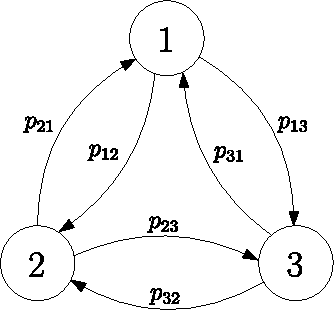
\includegraphics[width=0.35\textwidth]{figures/3_step_MC.pdf}}}$
	%\phantom{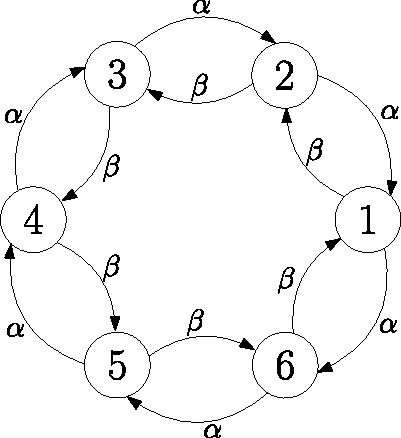
\includegraphics[width=0.1\textwidth]{figures/6_step_MC.pdf}}
	%$\vcenter{\hbox{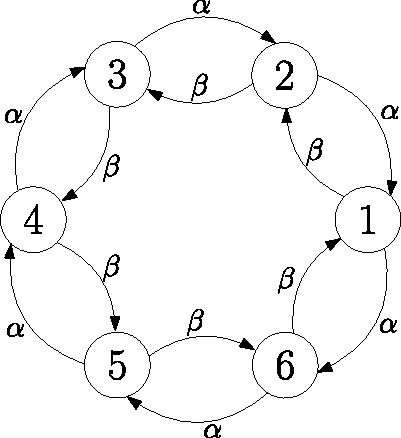
\includegraphics[width=0.35\textwidth]{figures/6_step_MC.pdf}}}$
	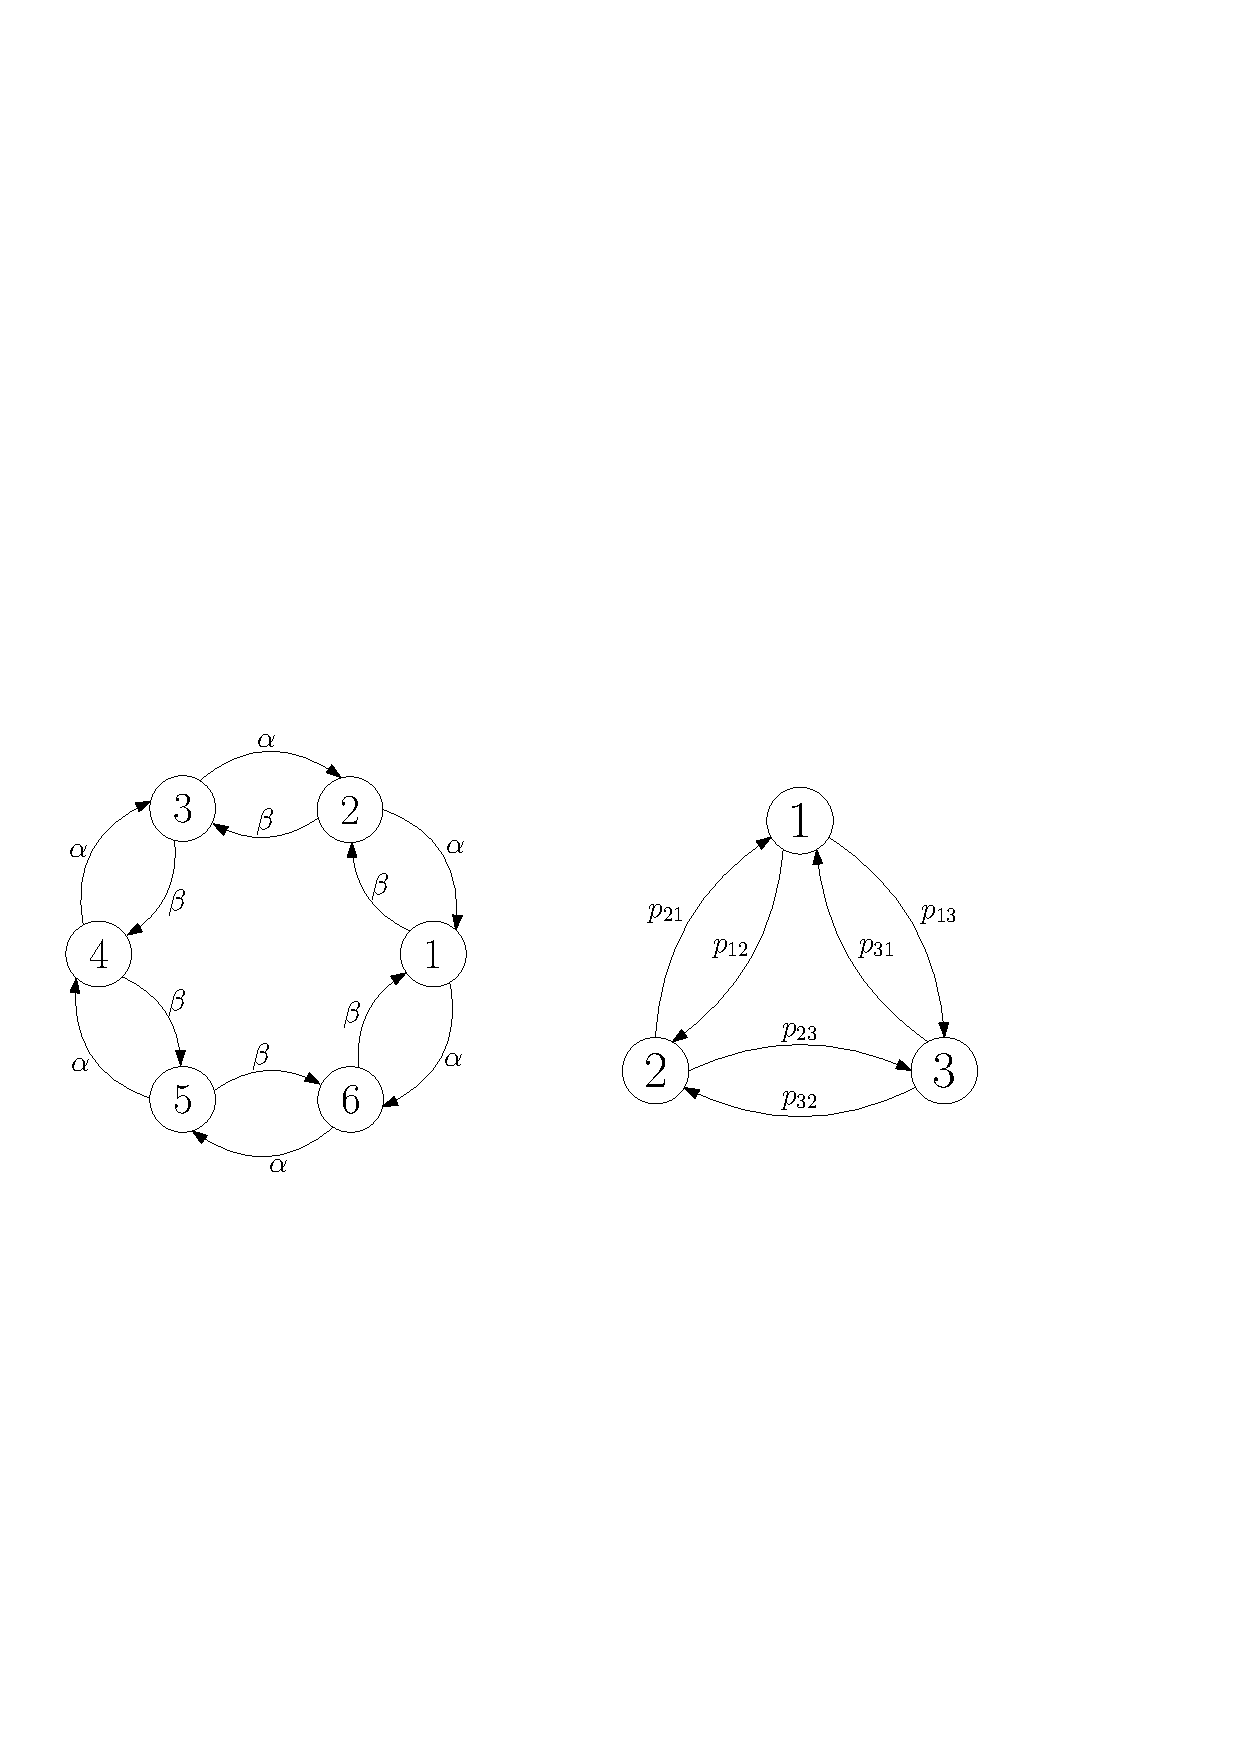
\includegraphics[width=\textwidth]{figures/n_step_MC.pdf}
\caption{6-State (asymmetric) Markov Chain and 3-State Markov Chain}
\end{figure}

\begin{defn}
	Let $p$ be a transition probability, $\mu$ a distribution on $E$, a sequence $(X_n)_{n\geq 0}$ of random variables with values in $E $ is a Markov Chain with initial distribution $\mu$ and transition probability $p$ (written $ \textrm{MC}(\mu, p)$) if for every $x_0, \ldots, x_n \in E$
\begin{align}
	\boxed{ \mathbb{P} \left[ X_0=x_0, \ldots ,X_n=x_n \right] = \mu(x_0)p_{x_0,x} \cdots p_{x_{n-1},x_{n}} .}
\end{align}
\end{defn}


\begin{prop}
	Let $X=(X_n)_{n \geq 0}$ sequence of random variables with values in $E$:
	\begin{align}
	X\textrm{ is a Markov Chain }\iff \exists \mu, p\textrm{ such that }X\textrm{ is a }MC(\mu, p)
	.\end{align}
	
\end{prop}
\begin{proof}
	$\implies:$ Define $\mu =$ law of $X_0$ and set 
	\begin{align}
		p_{xy} = 
	\begin{cases}
		\mathbb{P}_{} \left[ X_{n+1}=y | X_n -x \right] & \textrm{if } \exists n: \mathbb{P}_{} \left[ X_n = x \right] >0 \\
		\mathbbm{1}_{x=y} & \textrm{else}
	\end{cases}.
	\end{align}
	By homogeneity, $p_{xy}$ is well-defined. Furthermore, for every $x_0,\ldots,x_n \in E$ we have
\begin{align}
& \mathbb{P}_{} \left[ X_0=x_0, \ldots ,X_n=x_n \right] \\ 
	& \qquad = \mathbb{P}_{} \left[ X_n = x_n | X_0=x_0 , \ldots , X_{n-1}=x_{n-1} \right] \mathbb{P}_{} \left[ X_0=x_0 , \ldots , X_{n-1}=x_{n-1} \right] \\
	& \qquad = \mathbb{P}_{} \left[ X_0 = x_0 \right] \prod_{i=1}^{n} \mathbb{P}_{} \left[ X_i = x_i | X_0=x_0, \ldots , X_{i-1}=x_{i-1} \right] \\
	& \qquad = \mu(x_0) \prod_{i=1}^n \mathbb{P}_{} \left[ X_i = x_i | X_{i-1} = x_{i-1}  \right] = \mu(x_0) \prod_{i=1}^n p_{x_{i-1}x_{i}} 
.\end{align}
It remains to check that $p$ is a transition probability. Let $x \in E$. If there exists $n\geq 0$ such that $\mathbb{P}_{} \left[ X_n=x \right] >0$, then 
\begin{align}
	\sum_{y \in E}^{} p_{xy} = \sum_{y \in E}^{} \mathbb{P}_{} \left[ X_{n+1}=y | X_n =x \right] =1.
\end{align}
Otherwise,
\begin{align}
	\sum_{y \in E}^{} p_{xy} = \sum_{y \in E}^{} \mathbbm{1}_{x=y} =1
.\end{align}
$\impliedby:$ Assume  $(X_n)_{n\geq 0}$ is a MC$(\mu ,p)$. Let $n\geq 0$ and $x_0,\ldots,x_{n+1}$ such that $\mu (x_0) p_{x_0 x_1}\cdots p_{x_{n-1}x_n}>0$. We have that
\begin{align}
	\mathbb{P}_{} \left[ X_{n+1} = x_{n+1} | x_0 = x_0, \ldots, X_n = x_n \right] = \frac{\mathbb{P}_{} \left[ X_0 = x_0, \ldots, X_{n+1}= x_{n+1} \right] }{\mathbb{P}_{} \left[ X_0=x_0, \ldots, X_n = X_n \right] } = p_{x_nx_{n+1}}.
\end{align}
Now let $n\geq 0$ and $y \in E$ such that $\mathbb{P}_{} \left[ X_n = x \right] > 0$.
\begin{align}
&	\mathbb{P}_{} \left[ X_{n+1} = y | X_n =x \right] \\
&\qquad = \sum_{(u_0, \ldots ,u_{n-1}) \in E^n}^{} \mathbb{P}_{} \left[ X_{n+1}=y | X_0=u_0, \ldots ,X_{n-1}=u_{n-1}, X_n =x \right] \cdot \\
& \qquad \qquad \qquad \qquad \qquad  \mathbb{P}_{} \left[ X_0=u_0, \ldots , X_{n-1}=u_{n-1} | X_n = x \right] \\
&\qquad = p_{xy} \sum_{(u_0, \ldots ,u_{n-1})\in E^n}^{} \mathbb{P}_{} \left[ X_0=u_0, \ldots ,X_{n-1}=u_{n-1} | X_n = x \right] = p_{xy}
.\end{align}
This concludes that $X$ fulfills the two properties of a Markov Chain.

{\color{blue}
	$\implies:$ If $X_n$ is a Markov Chain, then set
	\begin{align}
		p_{xy} = 
	\begin{cases}
		\mathbb{P}_{} \left[ X_{n+1}=y | X_n -x \right] & \textrm{if } \exists n: \mathbb{P}_{} \left[ X_n = x \right] >0 \\
		\mathbbm{1}_{x=y} & \textrm{else}
	\end{cases}.
	\end{align}
	We have that $\sum_{y \in E}^{} p_{xy}=1$, as the conditional probability is a probability measure itself, and $p_{xy}\geq 0$, for every $x, y \in E$ for the same reason. Thus we have that the collection of $(p_{xy})_{x,y \in E}$ forms a transition probability. Setting $\mu(x) = \mathbb{P}_{} \left[ X_0 =x \right] $, which is also clearly a probability measure on $E$. Now we only have to show that $X_{n} $ is a $ \textrm{MC}(\mu, p)$. For every $x_0,\ldots , x_n \in E$, and every $n\geq 0$, we have
\begin{align}
& \mathbb{P}_{} \left[ X_0=x_0, \ldots ,X_n=x_n \right] \\ 
	& \qquad = \mathbb{P}_{} \left[ X_n = x_n | X_0=x_0 , \ldots , X_{n-1}=x_{n-1} \right] \mathbb{P}_{} \left[ X_0=x_0 , \ldots , X_{n-1}=x_{n-1} \right] \\
	& \qquad = \mathbb{P}_{} \left[ X_0 = x_0 \right] \prod_{i=1}^{n} \mathbb{P}_{} \left[ X_i = x_i | X_0=x_0, \ldots , X_{i-1}=x_{i-1} \right] \\
	& \qquad = \mu(x_0) \prod_{i=1}^n \mathbb{P}_{} \left[ X_i = x_i | X_{i-1} = x_{i-1}  \right] = \mu(x_0) \prod_{i=1}^n p_{x_{i-1}x_{i}} 
.\end{align}
Thus we have proven this implication by using the Markov property of Markov Chains.

$\impliedby:$ Here we have to demonstrate the two properties of a Markov Chain, the Markov property and homogeneity. For homogeneity we have
\begin{align}
&	\mathbb{P}_{} \left[ X_{n+1} = y | X_n =x \right] \\
&\qquad = \sum_{(u_0, \ldots ,u_{n-1}) \in E^n}^{} \mathbb{P}_{} \left[ X_{n+1}=y | X_0=u_0, \ldots ,X_{n-1}=u_{n-1}, X_n =x \right] \cdot \\
& \qquad \qquad \qquad \qquad \qquad  \mathbb{P}_{} \left[ X_0=u_0, \ldots , X_{n-1}=u_{n-1} | X_n = x \right] \\
&\qquad = p_{xy} \sum_{(u_0, \ldots ,u_{n-1})\in E^n}^{} \mathbb{P}_{} \left[ X_0=u_0, \ldots ,X_{n-1}=u_{n-1} | X_n = x \right] = p_{xy}
.\end{align}
here we have implicitly assumed that $\mathbb{P}_{} \left[ X_n = x \right] > 0$, as without this the conditional probability we are taking is not well-defined. In the case where this is not true, the fulfillment of the homogeneity property is trivial as the transition probability is constantly $1$.

For the Markov Property we have
\begin{align}
	\mathbb{P}_{} \left[ X_{n+1} = x_{n+1} | X_0 =x_0, \ldots ,X_n=X_n \right] &=
		\frac{\mathbb{P}_{} \left[ X_0=x_0, \ldots , X_{n+1}=x_{n+1} \right] }
		{\mathbb{P}_{} \left[ X_0=x_0 , \ldots , X_{n}=x_{n} \right]} \\
	&= \frac{\mu(x_0)p_{x_0 x_1}  \cdots  p_{x_{n}x_{n+1}}} {\mu(x_0)p_{x_0x_1} \cdots p_{x_{n-1}x_{n}}} \\
	&= p_{x_n x_{n+1}} = \mathbb{P}_{} \left[ X_{n+1} = x_{n+1} | X_n=x_n \right] 
.\end{align}
Where it is important to note that, again,  we have implicitly assumed that \newline $\mu(x_0)p_{x_0x_1} \cdots p_{x_{n-1}x_n}>0$. 
}
\end{proof}


\textbf{Question} Given $\mu, p$ does $ \textrm{MC}(\mu, p)$ always exist (as a Markov Chain)?

\section{Existence}

\begin{theorem}
	Let $p$ be a transition probability on $E$. Then there exist:
\begin{enumerate}
	\item a measurable space $(\Omega, F)$,
	\item a collection of probability measures $(\mathbb{P}_x)_{x}$ on $(\Omega, F)$, and
	\item a sequence of random variables $(X_n)_{n \geq 0}$ on $(\Omega, F)$ such that for all $x\in E$, under $P_x$, $(X_n)$ is  $ \textrm{MC}(\delta_x, p)$.
\end{enumerate}

\end{theorem}

\begin{proof}
	We first fix a measure $\mu $ on $E$ with $\mu (x)>0$ for every $x$ and construct a MC$(\mu,p)$ on some abstract probability space $(\Omega, \mathcal{F}, \mathbb{P}_{})$. Consider $X_0$ a random variable with law $\mu $, $U_1, U_2, \ldots$ i.i.d uniform random variable on  $[0,1]$. One can construct a measurable function $\Phi: E \times [0,1] \to E$ such that for any  $x \in E\ \mathbb{P}_{} \left[ \Phi(x,U)=y \right] = p_{xy}$. To achieve this, order $E=\{x_1, x_2, \ldots \}$ and define for every  $s_{i,j} = \sum_{k<j}^{} p_{x_ix_k}$ for every $i, j$, then set $\Phi(x_i, u) = x_j$ if $s_{ij}\leq u < s_{ij} p_{x_ix_j}$. Define by induction, for every $n\geq 0$ 
	\begin{align}
		X_{n+1} = \Phi(X_n, U_{n+1}).
	\end{align}
Then we have for every $x_0, \ldots, x_n \in E$ 
\begin{align}
	\mathbb{P}_{} \left[ X_0=x_0, \ldots ,X_n=x_n \right] &=
		\mathbb{P}_{} \left[ X_0=x_0, \Phi(x_0, U_1)=x_1 , \ldots , \Phi(x_{n-1}, U_{n}) = x_n \right] \\
	&= \mu(x_0)p_{x_0x_1} \cdots p_{x_{n-1}x_n}
\end{align}
Now define for every $x \in E$ $\mathbb{P}_{x}  = \mathbb{P}_{} \left[ \cdot | X_0 = x \right] $, this is well defined as $\mu (x)>0$. Then we have that for all $x \in E$ 
\begin{align}
	\mathbb{P}_{x} \left[ X_0 = x_0, \ldots, X_n = x_n \right] = \delta_x(x_0) p_{x_0 x_1} \cdots p_{x_{n-1}x_n}.
\end{align}

{\color{blue}
We consider a measure $\mu $ on $E$ such that for every $x \in E: \mu (x) >0$, some abstract probability space $(\Omega, \mathcal{F}, \mathbb{P} )$, let $X_0$ be a random variable with distribution $\mu $. Let $U_1,U_2, \ldots $ be i.i.d. uniform  random variables on $[0,1]$. Our goal is to use these uniform random variables to produce the probabilities given by the transition probabilities, in a way similar to Sklar's Theorem (knowledge of Sklar's is not needed here). To do this we enumerate $E=\{x_i, i> 0 \}$ and set $s_{ij}= \sum_{k<j}p_{x_ix_k} $. Note here that $s_{i,j+1}-s_{i,j} = p_{x_ix_j} $. Finally, set
\begin{align}
	\Phi: E \times [0,1] \to E;\ (x_i,u) \mapsto x_j \textrm{ if } u \in (s_{ij}, s_{i,j+1}]
.\end{align}
Now we have $X_0$ as needed and the tools to construct the sequence of random variables, along with the collection of probability measures we want.

We now have that $\mathbb{P}_{} \left[\Phi(x,U_1) = y  \right] = p_{xy}$. So if we set $X_{n+1} = \Phi(X_n, U_{n+1})$ for every $n>0$ (by induction), we find that
\begin{align}
	\mathbb{P}_{} \left[ X_0=x_0, \ldots ,X_n=x_n \right] &=
		\mathbb{P}_{} \left[ X_0=x_0, \Phi(x_0, U_1)=x_1 , \ldots , \Phi(x_{n-1}, U_{n}) = x_n \right] \\
	&= \mu(x_0)p_{x_0x_1} \cdots p_{x_{n-1}x_n}
,\end{align}
by independence.

Now if we define $\mathbb{P}_{x} $ as $\mathbb{P}_{} \left[\ \cdot\ | X_0 = x \right] $, then we have for every $x \in E$ that
\begin{align}
	\mathbb{P}_{x} \left[ X_0=x_0, \ldots ,X_n=x_n \right] = \delta_x(x_0)p_{x_0x_1} \cdots p_{x_{n-1}x_n}
.\end{align}
}
\end{proof}

\noindent
\textbf{Framework for the rest of the chapter} 
$E$ is finite or countable, $p$ transition probability, $(\Omega, \mathcal{F}, (P_x)_{x \in E})$ Probability Spaces, $(X_n)_{n \geq 0}$ random variables such that it is a  $ \textrm{MC}(\delta_x, p)$ under $P_x$.

For $\mu$ Prob measure on $E $ we write $\mathbb{P}_\mu = \sum_{x}\mu(x)\mathbb{P}_{x}$

\section{Simple Markov Property}
\begin{rmk}[]
Under $\mathbb{P}_\mu$, $X=(X_n)_{n \geq 0}$ is $ \textrm{MC}(\mu, p)$.
\begin{align}
	\mathbb{P}_\mu [X_{n+1}=x_{n+1} | X_0 = x_0, \ldots ,.X_n=x_n] = \mathbb{P}_\mu[X_{n+1}=x_{n+1}| X_n = x_n] = \mathbb{P}_{x_n}[X_1 =x_{n+1}]
\end{align}
i.e. conditional on $X_n=x$, $x_{n+1}$ is sampled like the first step of a $ \textrm{MC}(\delta_{x},p)$ independent of the past.
\end{rmk}
\textbf{Notation} $ \mathcal{F}_n = \sigma(X_0, \ldots ,X_n)$.

\begin{theorem}[Simple Markov Property (SiMP)]
	Let $\mu$ be a distribution on E. Let $x \in E, k \in \mathbb{N}$. For every $f: E^{\mathbb{N}} \to \mathbb{R}_+$ measurable and bounded, for every $Z$ bounded which is $ \mathcal{F}_k$ measurable random variable:
\begin{align}
	\boxed{	\mathbb{E}_\mu \left[ f((X_{k+n})_{n \geq 0})Z | X_k = x_k \right] = \mathbb{E}_{x_k} \left[ f((X_n)_{n \geq 0} \right] \mathbb{E}_\mu \left[ Z | X_k=x \right].} 
\end{align}
\end{theorem}
\begin{proof}
	First note that using $Z= \mathbbm{1}_{X_0=x_0, \ldots ,X_{k-1}=x_{k-1}}$ we only have to prove that 
\begin{align}
	\mathbb{E}_{\mu } \left[ f((X_{k+n})_{n\geq 0}) | X_0=x_0 , \ldots , X_k=x_k \right]= \mathbb{E}_{x_k} \left[ f((X_n)_{n\geq 0}) \right]
.\end{align}
We will proceed using {\color{blue} measure theoretic} induction. Approximate $f$ by step functions $f_k$, using linearity, we only have to show our claim for the function $\mathbbm{1}_{A} $ with $A \subset E ^{\mathbb{N}}$ measurable, i.e. 
	\begin{align}
	\mathbb{P}_{\mu } \left[ (X_{k+n})_{n\geq 0}\in A | X_0=x_0, \ldots ,X_k=x_k \right] = \mathbb{P}_{x_k} \left[ (X_n)_{n\geq 0} \in A \right] 
.\end{align}  
The collection of sets of the form $A=\{w \in E^{\mathbb{N}}: w_0=y_0, \ldots ,w_N=y_N\}$ for $N\geq 0$ and $y_0, \ldots ,y_N \in E$ form a $\pi $ system generating our $\sigma$-algebra. Furthermore, on such sets 
\begin{align}
&	\mathbb{P}_{\mu } \left[ (X_{k+n})_{n\geq 0}\in A | X_0 = x_0, \ldots ,X_k=x_k \right] \\
&\qquad= \mathbb{P}_{\mu} \left[ X_k=y_0, \ldots ,X_{k+N}= y_N | X_0=x_0, \ldots ,X_k=x_k  \right] \\
&\qquad= \frac{\mu (x_0) p_{x_0x_1} \cdots p_{x_{k-1}x_k} \delta_{x_k}(y_0)p_{y_0y_1} \cdots p_{y_{N-1}y_N}}{\mu (x_0) p_{x_0x_1} \cdots p_{x_{k-1}x_k} } \\
& \qquad= \delta_{x_k}(y_0)p_{y_0y_1} \cdots p_{y_{N-1}y_N} \\
& \qquad= \mathbb{P}_{x_k} \left[ (X_n)_{n\geq 0} \in A \right] 
.\end{align}
Dynkin's Lemma then allows us to extend this property to the entire $\sigma$-algebra.
\end{proof}


\begin{cor}
Let $\mu$ be a  distribution on $E$, $x \in E$, $k \in \mathbb{N}$, for all $f: E^{\mathbb{N}} \to \mathbb{R}$ measurable and bounded:
\begin{align}
	\boxed{	\mathbb{E}_\mu \left[ f((X_{k+n})_{n \geq 0} | X_k =x \right] = \mathbb{E} _x \left[ f((X_n)_{n \geq 0} \right] .}  
\end{align}
\end{cor}

\noindent
\section{n-Step Transition Probabilities}
\begin{defn}
	For every $n\geq0$, $x, y \in E$, define $p_{xy}^{(n)}=P_x[X_n=y]$
\end{defn}

\begin{prop}[Chapman Kolmogorov (CK)]
\begin{align}
	\forall m,n \geq 0 \ \forall x,y \in E \quad \boxed{ p_{xy}^{(m+n)}= \sum_{z \in E} p_{xz}^{(m)}p_{zy}^{(n)}.}
\end{align}
	
\end{prop}
\begin{proof}
Fix $m,n$ and $x,y \in E$.
	\begin{align}
		p_{xy}^{(m+n)} &\stackrel{\phantom{\textrm{(SiMP)}}}{=} 
			\mathbb{P}_{x} \left[ X_{m+n}=y \right] =
			\sum_{z \in E}^{} \mathbb{P}_{x} \left[ X_{m+n} | X_m = z \right] \mathbb{P}_{x} \left[ X_m = z \right] \\
		&\stackrel{\textrm{(SiMP)}}{=} \sum_{z \in E}^{} \mathbb{P}_{z} \left[ X_n=y \right] \mathbb{P}_{x} \left[ X_m=z \right] = \sum_{z \in E}^{} p_{xz}^{(m)} p_{zy}^{(n)}  	
	.\end{align}
	
\end{proof}


\begin{prop}[]
	If $E$ is finite:
The matrix $(p_{ij}^{(n)})_{ij \leq 0}$ is equal to $P^n$. for $\mu$ a distribution on $E$ the following holds for any $f:E \to \mathbb{R}$
	\begin{align}
	\mathbb{E}_{\mu} \left[ f(X_n) \right] = \mu P^n f
,\end{align}
for any $n\geq 0$, with $f = [f(1), \ldots ,f(n)]^T$.
\end{prop}
\begin{proof}
	The first equation follows from $p_{ik}^{(n+1)}= \sum_{j}^{} p_{ij}^{(n)}p_{jk}$ by induction. For the second equation, use the definition of the expectation
\begin{align}
	\mathbb{E}_{\mu } \left[ f(X_n) \right]  = \sum_{y \in E}^{}  f(y) \mathbb{P}_{\mu } \left[ X_n = y \right] = \sum_{x,y \in E^2}^{}  \mu (x) \underbrace{\mathbb{P}_{x} \left[ X_n =y \right]}_{=p_{xy}^{(n)}} f(y).
\end{align}
\end{proof}


\section{Stationary Distributions}
\textbf{Motivation}: write $\mu_{n}$ as the law of $X_{n}$ under $P_{\mu}$, $\mu_0=\mu$ and $\mu_{n+1}=\mu_{n}P$. For $n$ large $\mu_n$ is a fixed point of the map $\lambda \to \lambda P = \left( \sum_{x \in E} \lambda(z)p_{xy} \right)_{y \in E}$

\begin{defn}
	Let $\pi$ be a distribution on $E$, we say that $\pi$ is stationary (for $p$) if for $y \in E$
\begin{align}
	\boxed{ \pi(y) = \sum_{x \in E} \pi(x)p_{xy}.}
\end{align}

\textbf{Linear Algebra interpretation} If $E$ is finite and we write  $\pi = [\pi(1), \ldots ,\pi(n)]^T$, then 
\begin{align}
	\boxed{ \pi \textrm{ is stationary} \iff \pi P = \pi ,}
\end{align}
i.e. $\pi$ is a left eigenvector of P for the eigenvalue 1.

\textbf{Probabilistic interpretation} If $\pi $ is a stationary distribution, then for all $ n \geq 0$ 
\begin{align}
	P_{\pi }[X_n =x] = \pi (x)
.\end{align}
No matter how far along you are in the chain, the probability that you land on a value $x$ is equal to the probability that you start at $x$.
\end{defn}

\section{Reversibility}
\begin{defn}
	A distribution $\pi $ on $ E$ is said to be reversible (for $p$) if for any $x,y \in E$
\begin{align}
	\boxed{ \pi (x) p_{xy}= \pi (y)p_{yx}. }
\end{align}
The probability of starting at $y$ and going to $x$ is equal to the probability of starting at $x$ and going to $y$. More generally, one can prove by induction that $\pi $ is reversible $ \iff \forall n; \forall x_0, \ldots ,x_n: \mathbb{P}_{\pi } \left[ X_0=x_0, \ldots ,X_n=x_n \right] = \mathbb{P}_{\pi } \left[ X_0=x_n, \ldots ,X_n=X_0 \right] $.
\end{defn}

\textbf{Motivation} We want an easy criterion for invariance, such reversible systems appear often in physics.

\begin{prop}[]
	Let $\pi $ be a distribution on $E$, if $\pi $ reversible, then $\pi $ is stationary.
\end{prop}
\begin{proof}
	\begin{align}
		\sum_{x \in E}^{} \pi (x)p_{xy} = \sum_{x \in E}^{} \pi (y) p_{yx} = \pi (y) \sum_{x \in E}^{} p_{yx} = \pi(y) 
	.\end{align}	
\end{proof}

\begin{ex}[Gas in Containers (Ehrenfest Model)]
	Imagine there are two containers $A$ and $B$ with gas particles, between them is a small hole through which the particles can pass through. At every step a single particle is selected uniformly at random and passes through this hole. To represent this mathematically, let $X_n$ be the number of particles in $A$ at time $n$, and let there be $N$ total particles. We assume that the system in time homogeneous (time plays no role in its evolution, only its current state) and is memoryless (again only the current state of the system plays a role). This gives us the inspiration to model $X_n$ as a Markov Chain. The transition probabilities are given by $p_{x, x+1}= 1- \frac{x}{N}$, as in order for $X_n$ to grow by 1, the randomly selected particle must be from container $B $; this occurs with probability $\frac{\# \textrm{ of particles in }B}{\# \textrm{ of total particles}} = \frac{N-x}{N}$. The only other option is for the amount of particles in $A$ to decrease by 1, by the fact that the transition probabilities must sum to 1 we find: $p_{x, x-1}= \frac{x}{N}$. Now we wonder if it is possible to find a stationary distribution, this would represent the equilibrium distribution of particles (see the different interpretations above). To find this distribution, we instead simplify and see if we can find a reversible distribution, i.e. $\pi (x) p_{x,x+1} = \pi (x+1)p_{x+1, x}$. We then use this to calculate $\pi (x)$ explicitly and see if this defines a proper distribution. 
	\begin{align}
		\pi (x+1) = \frac{\pi (x)(1 - \frac{x}{N})}{\frac{x+1}{N}} = \pi (x) \frac{N-x}{x+1} \stackrel{\textrm{(Induction)}}{=} \pi (0) \frac{N  \cdots (N-x)}{(x+1)!} 
	.\end{align}	
	Thus we find that $\pi (x) = \binom{N}{x}\pi(0)$, $\pi$ should define a distribution. This entails that the total mass of $\pi $ be $1$, i.e. $\sum_{x \in E}^{} \pi (x)=1$. Hence we find 
\begin{align}
\pi (0) = \left( \sum_{x \in E}^{} \binom{N}{x} \right)^{-1} = \frac{1}{2^N} 
.\end{align}
Hence, $\pi (x)= \binom{N}{x} \frac{1}{2^N}$, the binomial distribution; which is (as we have shown) reversible. When $X_{n+1}$ is distributed like $X_n$ (equilibrium) then the number of particles in $A$ is distributed as $Bin(N, \frac{1}{2})$.
\end{ex}


\section{Communication Classes}
Here we will will see $p$ as a weighted oriented graph.
\begin{defn}
	Let $x,y \in E$. We say that "$y$ can be reached from $ x$" if there exists an $n \geq 0$ such that  $p_{xy}^{(n)}>0$ and we write $x \to y$. Furthermore, we say that "$x$ and $y $ communicate"  if $y$ can be reached from $x$ and $x$ can be reached from $y$, we write $x  \leftrightarrow y$.
\end{defn}

\begin{prop}[]
	$\leftrightarrow$ is an equivalence class on E
\end{prop}
\begin{proof}
	Let $x,y,z \in E$ and $m,n \geq 0$ such that $p_{xy}^{(m)}>0$ and $p_{yz}^{(n)}>0$.
\begin{enumerate}
	\item Transitivity: $p_{xz}^{(m+n)} \geq p_{xy}^{(m)}p_{yz}^{(n)} >0$ thus we know that $x\rightarrow z$, we can apply the same argument in the other direction as well. 
	\item Reflexivity: $p_{xx}^{(0)} = \mathbb{P}_{x} \left[ X_0 = x \right] =1>0$, hence $ x \leftrightarrow x$. 
	\item Symmetry: Trivial.
\end{enumerate}
\end{proof}


\begin{defn}
	The equivalence classes of $ \leftrightarrow $ are called communication classes, and if there is a single unique communication class for a chain $p$, we say that $p$ is irreducible.
\end{defn}

\noindent
\textbf{Motivation} We will see that $p$ irreducible implies that $p$ has at most one stationary distribution.

\begin{defn}
	A communication class $C$ is closed if for any $x,y \in E$
\begin{align}
 x \in C, x \to y \implies y \in C.
\end{align}
\end{defn}
"If you start in $C$ you never leave."

\section{Strong Markov Property}
%$F_n=\sigma(X_0, \ldots ,X_n)$ 
	
\begin{defn}
	Let $T:\Omega \to \mathbb{N} \cup \{+\infty\}$ random variable with values in $\mathbb{N}\cup\{+\infty\}$. We say that $T$ is an ($ \mathcal{F}_n$)-stopping time if for all $n \in \mathbb{N}$:
	\begin{align}
		\{T=n\} \in \mathcal{F}_n
	.\end{align}
\end{defn}

\begin{ex}[Stopping Times]
	$H_{A}=\min\{n \geq 0: X_n \in  A\}$ (for $A$ measurable) and $H_x=\min\{n\geq 0: X_n = x\}$ are stopping times.
\end{ex}

\begin{defn}
	Let $T$ be a stopping time. $ \mathcal{F}_T=\{A \in \mathcal{F}: \forall n \in \mathbb{N}: \{T=n\}\cap A \in \mathcal{F}_n \}$
\end{defn}

\begin{theorem}[Strong Markov Property (SMP)]
	Let $\mu $ be a distribution on $E$, $T$ an $ \mathcal{F}_n$-stopping time. Let $x \in E$,
	then for all $f:E^{\mathbb{N}} \to \mathbb{R}$ measurable and bounded, and $Z$ which are $ \mathcal{F}_T$ measurable and bounded, we have:
\begin{align}
	\boxed{ \mathbb{E}_{\mu } \left[ f((X_{T+n})_{n\geq 0}) \cdot Z | T<\infty, X_T=x \right] = \mathbb{E}_{x} \left[ f((X_n)_{n\geq 0}) \right]  \mathbb{E}_{\mu } \left[ Z | T<\infty, X_T=x \right].} 
\end{align}
\end{theorem}
\noindent
"Conditioned on $\{T<\infty,X_T=x\}$, $(X_{T+n})_{n\geq 0}$ is a $ \textrm{MC}(\delta_x,p)$ independent of $ \mathcal{F}_T$ "
\begin{proof}
We will multiply each side of the equation by $\mathbb{P}_{} \left[ T < \infty, X_T =x \right]$.
\begin{align}
&	\mathbb{E}_{\mu } \left[ f((X_{T+n})_{n\geq 0})Z \mathbbm{1}_{T<\infty, X_T=x}  \right] =
		\sum_{k\geq 0}^{} \mathbb{E}_{\mu } \left[ f((X_{k+n})_{n\geq 0} Z \mathbbm{1}_{T=k, X_T=k}  \right] \\
&\qquad	\stackrel{\phantom{\text{(SiMP)}}}{=}  \sum_{k\geq 0}^{} \mathbb{E}_{\mu } \left[ f((X_{k+n})_{n\geq 0}) Z \mathbbm{1}_{T=k} | X_k = x \right] \mathbb{P}_{\mu } \left[ X_k = x  \right] \\ 
&\qquad	\stackrel{\text{(SiMP)}}{=} \sum_{k\geq 0}^{} \mathbb{E}_{x} \left[ f((X_{n})_{n\geq 0}) \right] \mathbb{E}_{\mu } \left[ Z \mathbbm{1}_{T=k, X_k = x}  \right] \\
&\qquad	\stackrel{\phantom{\text{(SiMP)}}}{=} \mathbb{E}_{x} \left[ f((X_n)_{n\geq 0} \right] \sum_{k\geq 0}^{} \mathbb{E}_{\mu } \left[ Z \mathbbm{1}_{T=k, X_k=x}  \right]  
		= \mathbb{E}_{x} \left[ f((X_n)_{n\geq 0}) \right] \mathbb{E}_{\mu } \left[ Z \mathbbm{1}_{T<\infty, X_T=x}  \right] 
.\end{align}
\end{proof}


\noindent
\textbf{Application} Reflection Principle for the SRW.
\begin{figure}[h!]
\begin{center}
\begin{tikzpicture}
	\begin{axis}[ymajorgrids=true, grid style={line width=.3pt,  dashed}, enlargelimits={abs=0.5}, axis line style={latex-latex}, xticklabels={,},xtick={0,1,2,3,4,5,6,7,8,9}, ytick={-2,-1,0,1,2,3,4}, ymin=-2]
	\addplot[black,] coordinates { (0,0) (1,-1) (2,0) (3,1) (4,2) (5,1) (6,2) (7,3) (8,4) (9,3)}; 	
	\addplot[black, dashed] coordinates {(4,2) (5,3) (6,2) (7,1) (8,0) (9,1)};
\end{axis}
\end{tikzpicture}
\end{center}
\caption{Example of a reflected simple random walk for $a=2$}
\end{figure}

Consider the SRW on $\mathbb{Z}$: 

\begin{prop}[]
Let $k\geq 0$ even, $a\geq1$ odd: $\mathbb{P}_{0} \left[ \max_{0 \leq m \leq k} X_m \geq a \right] = \mathbb{P}_{0} \left[ |X_k|\geq a \right]  $
\end{prop}
\begin{proof}
	Define $H_a= \min\{n \geq 1: X_n =a\}$, this is a stopping time.
	\begin{align}
		\mathbb{P}_{0} \left[ \max_{0 \leq m \leq k}X_m \geq a \right] = \mathbb{P}_{0} \left[ H_a \leq k \right] = \mathbb{P}_{0} \left[ X_k > a \right]  + \mathbb{P}_{0} \left[ H_a \leq k, X_k < a \right] 
		.\end{align}		
		Now our goal is to show the term on the right is equal to $\mathbb{P}_{0} \left[ X_k > a \right] $, as $2\mathbb{P}_{0} \left[ X_k > a \right] = \mathbb{P}_{0} \left[ |X_k| >a \right] $ by symmetry. We can go from $>$ to $\geq$ because $a$ is even and $k$ is odd. At this point we note that $X_{H_a +n}$ is distributed as $a + (a-X_{H_a +n}) = 2a - X_{H_a +n}$. Geometrically, this means that if we only look at the walk after hitting $a$, the walk has the same distribution if we inverse the direction of each step: 'looking at the path after hitting $a$, we cannot tell if it is the normal or the inverted step walk'.
	\begin{align}
		\mathbb{P}_{0} \left[ H_a \leq k, X_k < a \right] &= \sum_{m=0}^{k} \mathbb{P}_{0} \left[ X_k < a, H_a = m \right] = \sum_{m=0}^{k} \mathbb{P}_{a} \left[ X_{k-m} < a \right] \mathbb{P}_{0} \left[ H_a = m \right]  \\
		&= \sum_{m=0}^{k} \mathbb{P}_{a} \left[ X_{k-m}>a \right] \mathbb{P}_{0} \left[ H_a = m \right] = 
			 \sum_{m=0}^{k} \mathbb{P}_{0} \left[ X_{k-m}>a, H_a =m \right] \\
		&= \mathbb{P}_{0} \left[ X_k >a, H_a \leq k \right] = \mathbb{P}_{0} \left[ X_k > a \right]  
	 .\end{align}	
\end{proof}


\noindent
\textbf{Conclusion} Now we have properly defined a Markov Chain, shown its existence, and introduced some concepts to help classify different types of chains. Importantly, we have also introduced the transition probability framework. 



\newpage

\chapter{Markov Chains: Long Time Behavior}
\noindent \textbf{Outset} With the tools and classification concepts introduced previously, we would like to expand upon these to rigorously classify chains.

\noindent \textbf{Framework:} $E$ finite or countable, $p=(p_{xy})x,y \in E$ transition probabilities, ($\Omega, F, (\mathbb{P}_x) _{x \in E}$), $X=(X_n)_{n\geq 0} \sim MC(\delta_x,p)$ under $\mathbb{P}_x$, $\mathbb{P}_\mu = \sum_{}^{} \mu (x)\mathbb{P}_x$.

\noindent \textbf{Questions:} 
\begin{itemize}
	\item When does there exist a stationary distribution?
	\item What is the behavior of $X_n$ for $n$ large?
	\item If we fix $x \in E$, will the chain visit $x$ infinitely many times?
\end{itemize}

\section{Recurrence/Transience}

\textbf{Notation} $H_x = \min\{n\geq 1: X_n=x\}$
\begin{defn}
	Let $x \in E$, we say that:
\begin{itemize}
	\item $x$ is recurrent if $\boxed{\mathbb{P}_{x} \left[ H_x<\infty \right]=1 }$.
	\item $x$ is transient if $\boxed{\mathbb{P}_{x} \left[ H_x<\infty \right] <1}$.
\end{itemize}

\end{defn}
\noindent
\textbf{Notation:} For $x \in E$ write $V_x=\sum_{n\geq 0}^{} \mathbbm{1}_{X_n=x} $, ie the total number of visits.

\begin{theorem}[Dichotomy Theorem]
	$x \in E$:
\begin{itemize}
	\item if $x$ is recurrent, then $\boxed{V_{x}=+\infty} \ P_x$-a.s..
	\item if $x$ is transient, then $\boxed{\mathbb{E}_{x} \left[ V_x \right] <\infty}$.
\end{itemize}
\end{theorem}

\begin{rmk}[]
It is impossible that $\mathbb{P}_{x} \left[ V_x<\infty \right] >0 $ and $\mathbb{E}_{x} \left[ V_x \right] =+\infty$.
\end{rmk}


\begin{defn}
	$\rho_x = \mathbb{P}_{x} \left[ H_x<\infty \right]$, if $x$ is recurrent then $\rho_x=1$, otherwise if $x$ is transient $\rho_x<1$. Thus the number of visits is a geometric RV with parameter $\rho_x<1$.
\end{defn}

\begin{lemma}[]
	For every $i\geq 0, x \in E$, we have $\mathbb{P}_{x} \left[ V_x \geq i \right] = \rho_x^{i}$.
\end{lemma}

\begin{proof}[Proof (Lemma)]
	We will proceed by induction over $i$. Define $H_x^{(i)}$ to be the $i$-th hit time of $x$. For $i=0$ the claim is clear.
	\begin{align}
		\mathbb{P}_{x} \left[ V_x \geq i+1 \right] &\stackrel{\phantom{\text{(SMP)}}}{=} \mathbb{P}_{x} \left[ V_x \geq i+1, V_x \geq i \right] = \mathbb{P}_{x} \left[ H_x^{(i_1)} < \infty, H_x^{(i)} < \infty \right] \\
		&\stackrel{\phantom{\text{(SMP)}}}{=} \mathbb{P}_{x} \left[ H_x^{(i+1)} < \infty | H_x^{(i)} < \infty, X_{H_x^{(i)}}=x \right] \mathbb{P}_{x} \left[ H_x^{(i)} < \infty \right] \\
		&\stackrel{\text{(SMP)}}{=} \mathbb{P}_{x} \left[ H_x^{(1)} < \infty \right] \rho_x^i = \rho_x^{i+1}   
	.\end{align}
\end{proof}

\begin{proof}[Proof (Theorem)]
	For $x$ recurrent: 
	\begin{align}
		\mathbb{P}_{x} \left[ V_x = \infty \right] = \mathbb{P}_{x} \left[ \bigcap_{i=0}^{\infty} \{V_x \geq i\} \right] = \lim_{i\to \infty} \mathbb{P}_{x} \left[ V_x \geq i \right] = \lim_{i \to \infty} \rho_x^{i} = 1 
	.\end{align}
	For $x$ transient:
	\begin{align}
		\mathbb{E}_{x} \left[ V_x \right] &= \sum_{k=0}^{\infty} k \mathbb{P}_{x} \left[ V_x = k \right] = \sum_{k=1}^{\infty} \sum_{j=1}^{k} \mathbb{P}_{x} \left[ V_x=k \right] = \sum_{j=1}^{\infty} \sum_{k=j}^{\infty} \mathbb{P}_{x} \left[ V_x=k \right] \\
	&= \sum_{j=1}^{\infty} \mathbb{P}_{x} \left[ V_x \geq j \right] = \sum_{j=1}^{\infty} \rho_x^k = \frac{\rho_x}{1-\rho_x} < \infty
	.\end{align}
\end{proof}

\begin{prop}[]
	If $E$ is finite, then there exists a recurrent state $x \in E$.
\end{prop}
\begin{proof}
	Fix some $y \in E$.
	\begin{align}
		\sum_{x \in E}^{} V_x = \sum_{n=0}^{\infty} \sum_{x \in E}^{} \mathbbm{1}_{X_n =x} = \sum_{n\geq 0}^{} 1  = \infty \\
	\sum_{x \in E}^{} \mathbb{E}_{y} \left[ V_x \right] = \mathbb{E}_{y} \left[ \sum_{x \in E}^{} V_x \right] = \infty 
.	\end{align}

	Thus we know there exists $x \in E$ such that $\mathbb{E}_{y} \left[ V_x \right] = \infty$ since the sum on the left is over a finite index set ($E$ finite). Since we can write $V_x = V_x \mathbbm{1}_{H_x<\infty}$, we find that (using the Strong Markov Property) 
\begin{align}
	\infty = \mathbb{E}_{y} \left[ V_x \right] = \mathbb{E}_{y} \left[ V_x \mathbbm{1}_{H_x<\infty}  \right] = \mathbb{E}_{x} \left[ V_x \right] \mathbb{P}_{y} \left[ H_x < \infty \right] 
,\end{align}
	 because a walk started from $y$ is the same (in the distribution sense) after hitting $x$ as a walk started from $x$. $\mathbb{P}_{y} \left[ H_x < \infty \right]$ must be $ \leq 1 $, thus the term of the left must be equal to $\infty$, implying that $\mathbb{E}_{x} \left[ V_x \right] = \infty$.
\end{proof}


\section{Recurrence/Transience for the SRW on $\mathbb{Z}^d$}
\textbf{SRW on $\mathbb{Z}^d$:} $E=\mathbb{Z}^d$, $p_{xy}=\frac{1}{2d}\ if\ \|x-y\|_1=1, 0\ else$ 

\begin{theorem}[Polya]
	For the SRW, every state is recurrent if $d=1,2$, otherwise they are transient.
\end{theorem}
\begin{proof}
	Let $(Z_k)_{k> 0}$ be i.i.d. random variables on some probability space $(\Omega, \mathcal{F}, \mathbb{P})$ with $\mathbb{P}_{} \left[ Z_i = \pm e_i \right] = \frac{1}{2d}$ for $i= 1 \ldots d$ and $e_i$ being the unit vectors in $\mathbb{Z}^{d}$. Next, define $X_n = \sum_{k=1}^{n} Z_k$, which is a $MC(\delta_0, p)$. Then we find the following
	\begin{align}
		\mathbb{E}_{} \left[ V_i \right] = \mathbb{E}_{} \left[ \sum_{n> 0}^{} \mathbbm{1}_{X_n =0}  \right] = \sum_{n> 0}^{} \mathbb{P}_{} \left[ X_n = 0 \right] .
	\end{align}
	\textbf{Idea:} $\mathbb{P}_{} \left[ X_n=x \right]  = \mathbb{P}_{} \left[ Z_1+ \ldots + Z_n = x \right] = \sum_{\delta_1 + \ldots + \delta_n =x}^{} \mathbb{P}_{} \left[ Z_1 = \delta_1 \right] \cdots \mathbb{P}_{} \left[ Z_n = \delta_n \right]  $ is not easy to calculate. Instead, we use could use the Fourier Transform to link $\mathbb{E}_{} \left[ e^{i X_n} \right] = \mathbb{E}_{} \left[ e^{iZ_1} \right] ^n $ to $(\mathbb{P}_{} \left[ X_n =x\right] )_{x \in \mathbb{Z}^d}$.
	Define $\phi(\xi) = \mathbb{E}_{} \left[ e^{i \xi \cdot Z_1} \right] $ for $\xi$ in $\Pi^d = [-\pi, \pi)^d$. Then we have
	\begin{align}
		\phi(\xi) = \frac{1}{2d} \sum_{i=1}^{d} (e^{i \xi \cdot e_1} + e^{i \xi \cdot e_1}) = \frac{1}{d} \sum_{i=1}^{d} \cos(\xi_i)
	.\end{align}
	Fixing $n\geq 0$, we have (by independence) that the characteristic function of $X_n$ is 
	\begin{align}
		\varphi_{X_n}(\xi) = \mathbb{E}_{} \left[ e^{i \xi \cdot X_n} \right]  = \mathbb{E}_{} \left[ e ^{i ( \xi \cdot Z_1 + \ldots + \xi \cdot Z_n)} \right] = \phi(\xi)^n. 	
	\end{align}
We can now take advantage of the Fourier Transform by using the Fourier inversion, giving
\begin{align}
	\mathbb{P}_{} \left[ X_n = 0 \right] = \frac{1}{(2 \pi) ^d} \int_{\Pi^d}^{} \phi(\xi)^n d\xi.
\end{align}
Check this by directly computing
\begin{align}
	\int_{[0, 2\pi)^d}^{} \phi(\xi)^n d\xi &= \int_{[-\pi, \pi)^d}^{} \sum_{x \in \mathbb{Z}^d}^{} \mathbb{P}_{} \left[ X_n = x \right] = \sum_{x \in \mathbb{Z}^d}^{} \mathbb{P}_{} \left[ X_n = x \right] \int_{[0, 2 \pi)^d}^{} e^{i \xi \cdot x} d\xi  \\
	&= 
	\begin{cases}
		(2 \pi)^d & \textrm{if }x = 0 \\
		0 & \textrm{if } x \neq 0
	\end{cases}.
\end{align}
Therefore,
\begin{align}
	(2 \pi )^d \sum_{n\geq 0}^{} \mathbb{P}_{} \left[ X_n =0 \right] 
		&\stackrel{\phantom{\textrm{(Fub)}}}{=} \sum_{n> 0}^{} \int_{\Pi^d}^{} \phi(\xi)^n d \xi 
		\stackrel{\textrm{(MCT)}}{=} \lim_{\alpha \uparrow 1} \sum_{n> 0}^{} \int_{\Pi^d}^{} (\alpha \phi(\xi))^n d\xi \\
	& \stackrel{\textrm{(Fub)}}{=} \lim_{\alpha \uparrow 1} \int_{\Pi^d}^{}  \frac{1}{1-\alpha \phi(\xi)} d \xi 
		\stackrel{\textrm{(MCT)}}{=} \int_{\Pi^d}^{} \frac{1}{1-\phi(\xi)} d \xi
.\end{align}
We can see that for any $\xi_i \in [-\pi, \pi )$ we have the inequality $\frac{\xi_i^2}{6} \leq 1 - \cos(\xi_i) \leq \frac{\xi_i^2}{2}$. 

With this, we find that $\frac{1}{6d}\| \xi \|_2^2 \leq 1 - \phi(\xi) \leq \frac{1}{2d} \| \xi \|_2^2$, finally giving us
\begin{align}
	\sum_{n\geq 0}^{} \mathbb{P}_{} \left[  X_n = 0\right] < \infty \iff \int_{B_1(0)}^{} \frac{d\xi}{\| \xi \|_2^2} < \infty \iff d>2.
\end{align}
The final equivalence can be justified by using a change of variables and homogeneity. Define $A_i = B_0(2^{-i}) \setminus B_0(2^{-(i+1)})$ for every $i$. Next use the change of variable $\psi = 2^{i}\xi$, we find that
\begin{align}
	\int_{A_i}^{} \frac{d\xi}{\| \xi \|^2} = \int_{A_0}^{} \frac{2^{2i}}{\| \psi \|^2} (2^{i})^{-d} d\psi
	= (2^{i})^{2-d} \underbrace{ \int_{A_0}\frac{d\psi}{\| \psi\|^2}}_{=: I_0}.
\end{align}
Therefore 
\begin{align}
	\int_{B_0(1)}^{} \frac{d \xi}{\| \xi \|^2} = \sum_{i=0}^{\infty} \int_{A_i}^{} \frac{d\xi}{\| \xi\| ^2} = I_0 \sum_{i=0}^{\infty} (2^i)^{2-d}.
\end{align}
Which is finite if and only if $d>2$.
\end{proof}

\section{Classification of States}
\begin{theorem}[]
	Let $x,y \in E$ such that $x \to y$. If $x $ is recurrent then $y$ is recurrent and $\mathbb{P}_{x} \left[ H_y<\infty \right] = \mathbb{P}_{y} \left[ H_x<\infty \right]=1 $.
	In particular $x \leftrightarrow y$.
\end{theorem}
\begin{proof}
	We want to use that every time the chain visits $x$, it has a non-zero probability to visit $y$ after that, visiting $x$ infinitely often should ensure that $y$ is also visited infinitely often.
	Assume $y \neq x$ and $x$ recurrent. Let $z_1, \ldots, z_{k-1}$ be distinct elements of $E$, not equal to $x$ or $y$ such that $p_{xz_1}\cdots p_{z_{k-1}y}>0$. Then we have
	\begin{align}
		0 &\stackrel{\phantom{\textrm{(SiMP)}}}{=} \mathbb{P}_{x} \left[ H_x = \infty \right]  
			> \mathbb{P}_{x} \left[ X_1=z_1, \ldots, X_k=1, \forall n> 0\ X_{k+n} \neq x \right]  \\
		  &\stackrel{\textrm{(SiMP)}}{=} \underbrace{\mathbb{P}_{x} \left[ X_1 = z_1, \ldots, X_k=y \right]}_{>0}
		  \underbrace{\mathbb{P}_{y} \left[ \forall n> 0\ X_n \neq x \right]}_{\mathbb{P}_{y} \left[ H_x = \infty \right]}  
	.\end{align}
Thus $\mathbb{P}_{y} \left[ H_x < \infty \right] =1$.
Next, we have to show that $y$ is recurrent. Choose $m,n$ such that $p_{xy}^{(n)}, p_{yx}^{(m)}>0$, we have
\begin{align}
	\mathbb{E}_{y} \left[ V_y \right] = \sum_{k> 0}^{} p_{yy}^{(k)} \geq \sum_{k> 0}^{} p_{yy}^{(m+k+n)} \stackrel{\textrm{(CK)}}{\geq} \underbrace{p_{yx}^{(m)}}_{>0} \underbrace{\left( \sum_{k> 0}^{} p_{xx}^{(k)} \right)}_{=\infty} \underbrace{ p_{xy}^{(n)}}_{> 0}.
\end{align}
Hence, $y$ is recurrent. To show that $\mathbb{P}_{x} \left[ H_y < \infty \right] = 1$, use the same argument as above, but with the roles of $x$ and $y$ swapped ($y \to x,\ y$ recurrent).
\end{proof}


\begin{rmk}[]
	$x \neq y: x \to y$ if and only if $\mathbb{P}_{x} \left[ \exists n: X_n=y \right]>0$ if and only if $ \mathbb{P}_{x} \left[ H_y<\infty \right]=1 $
\end{rmk}

\begin{cor}[]
	Let $C$ communication class for p. Either $x$ is recurrent for every $x \in E$, or every $x \in E$ is transient.
\end{cor}
\begin{proof}
	If $x  \leftrightarrow y $, we have that $x$ recurrent if and only if $y$ is recurrent.
\end{proof}
\begin{rmk}[]
	We call a class which is comprised of recurrent states a recurrent class, and one comprised of transient states a transient class.
\end{rmk}


\begin{cor}[]
	A recurrent class is always closed.
\end{cor}
\begin{proof}
	$C$ recurrent, $x \in C$, if $x \to y$ then we must have $y \to x$ (otherwise $x$ wouldn't be recurrent), therefore $y \in C$.
\end{proof}
\begin{cor}[]
	Thus we have an intuitive criterion for transience: if $x \to y$ but $y  \nrightarrow x$, then $x$ is transient. 'If we start at  $x$ and can get to a state, from which we cannot return to $x$, then $x$ is transient'.
\end{cor}

\begin{rmk}[]
	In general it is possible to find disjoint subsets of $E$ $T$ and $R_k$ such that $T$ is the class of transient states, and $R_k$ are recurrent classes, with $E = T \cup \bigcup_{k\geq 0}R_k$. Then we can broadly classify the behavior of the chain by differentiating if $X_n$ starts in some $R_k$, in which case the chain remains in $R_k$ forever, and if $X_n$ starts in $T$. If $X_n$ starts in $T$, either it remains in $T$ forever, or at some point it moves into an $R_k$ and remains there forever.
\end{rmk}


\section{Positive/Null Recurrence}
\textbf{Notation} For $x \in E$ write $m_{x}=\mathbb{E}_{x} \left[ H_x \right] $.

\begin{defn}
	Let $x \in E$ be a recurrent state. We say that $x$ is:
\begin{itemize}
	\item positive recurrent if $\boxed{m_x<\infty}$ 
	\item null recurrent if $\boxed{m_x=+\infty}$.
\end{itemize}

\end{defn}

\begin{theorem}[]
	Let $x,y \in E, x \leftrightarrow y$. Then 
	\begin{align}
	\boxed{\lim_{n \to \infty}\frac{1}{n}\sum_{k=1}^{n} p_{xy}^{(k)}=\frac{1}{m_{y}}}
	.\end{align}
\end{theorem}
\begin{rmk}[]
	Write $V_{y}^{(n)}=\sum_{k=1}^{n} \mathbbm{1}_{X_k=y}$, "The number of visits to $y$ up to time $n$". Thus the sum in the theorem is "Expected proportion of time spent at $y$".
\end{rmk}

If $y$ is transient, or null recurrent ($m_y=\infty$), the theorem tells us that $\lim_{n \to \infty}\mathbb{E}_{x} \left[ \frac{V_y^{(n)}}{n} \right] =0$: "null density of visits". Otherwise, $y$ is positive recurrent and the expected density of visits is strictly positive.

\begin{defn}[inter-visit times]
	Let $y \in E$. Define $H_y^{0}=H_y$ and for all $i\geq 1: H_{y}^{i}= \min\{n \geq 1: X_{H_y^0 +  \ldots  + H_y^{i-1}+n}=y\}$ if $H_y^{i-1}<\infty$, else $+\infty$	
\end{defn}
TODO: Figure would be good here

\begin{lemma}[]
	Let $x,y$ with $x \leftrightarrow y$, assume $y$ is recurrent. Then for every $j \geq 1$ and $t_0, \ldots, t_j \in \mathbb{N}$:
\begin{align}
	\mathbb{P}_{x} \left[ H_y^0=t_0 \ldots H_y^j=t_j \right] = \mathbb{P}_{x} \left[ H_y=t_0 \right] \mathbb{P}_{y} \left[ H_y=t_1 \right]  \ldots  \mathbb{P}_{y} \left[ H_y=t_j \right] 
\end{align}
Under $P_x$, $H_y^1,H_y^2, \ldots $ are i.i.d. with law $\mathbb{P}_{x} \left[ H_y^i=t \right] = \mathbb{P}_{y} \left[ H_y=t \right] $.
\end{lemma}
\begin{proof}
	Write $H^i = H_y^i$, we will prove via induction over $j$. We have $\mathbb{P}_{x} \left[ H^0 = t \right]  = \mathbb{P}_{x} \left[ H_y = y \right] $ for all $t$, showing for $j=0$.
	$j \to j+1$: First note that 
	\begin{align}
	\mathbb{P}_{x} \left[ H^0 < \infty, \ldots, H^j < \infty \right] = \sum_{t_0,\ldots, t_j}^{} \mathbb{P}_{x} \left[ H^0 = t_0, \ldots, H^j=t_j \right] = \mathbb{P}_{x} \left[ H_y < \infty \right] \mathbb{P}_{y} \left[ H_y < \infty \right] ^j = 1.
	\end{align}
	Therefore $T = H^0 + \ldots + H^j$ is finite $\mathbb{P}_{x} $-a.s. and $X_T=y$. Hence, we have that for every $t_0,\ldots,t_{j+1} \in \mathbb{N}$ that
	\begin{align}
		\mathbb{P}_{x} \left[ H^0=t_0,\ldots,H^{j+1}=t_{j+1} \right] &\stackrel{\phantom{\textrm{(SMP)}}}{=} \mathbb{P}_{x} \left[ H^0 = t_0, \ldots, H^{j+1}=t_{j+1} | T<\infty, X_T = y \right]  \\
		&\stackrel{\textrm{(SMP)}}{=} \mathbb{P}_{x} \left[ H^0=t_0, \ldots, H^j=t_j \right] \mathbb{P}_{y} \left[ \min\{n> 0: X_n =y\} = t_{j+1} \right] \\ 
	&\stackrel{\phantom{\textrm{(SMP)}}}{=} \mathbb{P}_{x} \left[ X_y = t_0 \right] \mathbb{P}_{y} \left[ H_y = t_1 \right] \cdots \mathbb{P}_{y} \left[ H_y = t_{j+1} \right]  
	.\end{align}
\end{proof}

\begin{proof}[Proof (Theorem)]
	\textbf{Case 1:} $y$ transient:	we know that $\mathbb{E}_{y} \left[ V_y \right] < \infty$, thus (Strong Markov Property) $\mathbb{E}_{x} \left[ V_y \right] < \infty$. Hence,
	\begin{align}
		\frac{\mathbb{E}_{x} \left[ V_y^{(n)} \right] }{n} \leq \frac{\mathbb{E}_{x} \left[ V_x \right] }{n} \to 0
	.\end{align}
	\textbf{Case 2:} $y$ recurrent: using the lemma, we know that the random variables $H^j$ are i.i.d. under $\mathbb{P}_{x}$ and fulfill $\mathbb{E}_{x} \left[ H^1 \right] = \mathbb{E}_{y} \left[ H_y \right]  = m_y$. Then we can use the Law of Large Numbers and $\mathbb{P}_{x} \left[ H^0 < \infty \right] =1$ we find $\mathbb{P}_{x}$-a.s.,
	\begin{align}
		\lim_{i\to \infty } \frac{H^0 + \ldots + H^i}{i} = m_y
	.\end{align}
	It should be noted that this includes the case of $m_y=\infty$ by truncation. Now we write $N_n = V_y^{(n)}$ (the number of visits to $y$ at time $n$).

	TODO: Figure

Following directly from the definition of $N_n$ we have that for any $n> 0$ that 
\begin{align}
	H^0 + \ldots + H^{N_n -1} \leq n < H^0 + \ldots + H^{N_n}
.\end{align}
Hence, for every $n> 0$ 
\begin{align}
\frac{N_n}{H^0 + \ldots H^{N_n}} < \frac{V_y^{(n)}}{n} \leq \frac{N_n}{H^0 + \ldots + H^{N_n -1}} 
.\end{align}
The upper and lower bounds each converge to $\frac{1}{m_y}$ almost surely. Hence, we can conclude that $\mathbb{E}_{x} \left[ \frac{V_y^{(n)}}{n} \right] \to \frac{1}{m_y}$ by the Dominated Convergence Theorem.
\end{proof}


\begin{prop}[Classification of recurrent classes]
	Let $R$ be a recurrent class. Then either:
\begin{itemize}
	\item For all $x \in R,\ x$ is positive recurrent
	\item For all $x \in R,\ x$ is null recurrent.
\end{itemize}
\end{prop}
\begin{proof}
	Fix $x,y \in E$ with $x  \leftrightarrow  y$ and $x$ recurrent. Fix $k\geq 0$ with $p_{xy}^{(k)}>0$. By Chapman-Kolmogorov, we have for all $j> 0$
	\begin{align}
		p_{xy}^{(k+j)} \geq p_{xx}^{(j)} p_{xy}^{(k)}	
.	\end{align}
Thus	
\begin{align}
	\underbrace{\frac{1}{n} \sum_{i=1}^{n} p_{xy}^{(i)}}_{\to  \frac{1}{\mathbb{E}_{y} \left[ H_y \right] }} \geq \underbrace{\left( \frac{1}{n} \sum_{j=1}^{n-k} p_{xx}^{(j)} \right)}_{\to \mathbb{E}_{x} \left[ H_x \right]} \underbrace{p_{xy}^{(k)}}_{>0}
.\end{align}
Therefore, $\frac{1}{\mathbb{E}_{y} \left[ H_y \right] }> 0$ and $y$ is recurrent.
\end{proof}


\begin{prop}[]
	Let $R$ be a recurrent class, if $R$ is finite, then $R$ is positive recurrent.
\end{prop}
\begin{proof}
	Fix $x\in R$, since $R$ is closed we have for every $n> 0$
	\begin{align}
		1 = \mathbb{P}_{x} \left[ X_n \in R \right] = \sum_{y\in R}^{} p_{xy}^{(n)}.
	\end{align}
Hence, 
\begin{align}
	1 = \sum_{y\in R}^{} \frac{1}{n} \sum_{k=1}^{n} p_{xy}^{(k)} \to \sum_{y \in R}^{} \frac{1}{\mathbb{E}_{y} \left[ H_y \right] }.
\end{align}
Thus, there must be a $y\in R$ such that $\mathbb{E}_{y} \left[ H_y \right] < \infty $, implying that the entire class is positive recurrent.
\end{proof}


\section{Stationary Distributions for Irreducible Chains}
\begin{theorem}[]
	Assume that $p$ is irreducible. 
\begin{itemize}
	\item If the chain is transient or null recurrent, then there is no stationary distribution;
	\item if the chain is positive recurrent, then there exists a unique stationary distribution given by 
		\begin{align}
		\boxed{\pi (x) = \frac{1}{\mathbb{E}_{x} \left[ H_x \right] }}
		.\end{align}
		
\end{itemize}
\end{theorem}
\begin{proof}
	We will begin by assuming a stationary distribution $\pi$ exists. Then for every $x \in E$ we have for all $n> 0$
	\begin{align}
		\pi (x) = \frac{1}{n} \sum_{k=1}^{n} \mathbb{P}_{\pi } \left[ X_k=x \right]  = \sum_{y \in E}^{} \pi(y) \frac{1}{n} \sum_{k=1}^{n} \mathbb{P}_{y} \left[ X_k = x \right] \to \sum_{y \in E}^{} \pi (y) \frac{1}{\mathbb{E}_{x} \left[ H_x \right] }	
	.\end{align}	
	Note that this also shows uniqueness of the stationary distribution.

	Now if we assume that the chain is transient or null recurrent, then using Dominated Convergence Theorem, we have that $\pi (x) = \frac{1}{\mathbb{E}_{x} \left[ H_x \right] } = 0$. This is a contradiction to $\sum_{x \in E}^{} \pi (x) = 1$, therefore no stationary distribution can exist.
	If, instead, we assume that the chain is positive recurrent, we have the same formula as before for $\pi (x)$ as the only possible candidate for the stationary distribution. So if we can show that $\pi $ indeed defines a stationary distribution (unlike in the previous case), then we will be done. First, we fix $x> 0$ and find the inequality for all $y \in E$ 
\begin{align}
\frac{1}{\mathbb{E}_{y} \left[ H_y \right] } &\stackrel{\phantom{\textrm{(Fatou)}}}{=} \lim_{n\to \infty} \frac{1}{n} \sum_{j=k}^{n} p_{yy}^{(j)} \\
					     &\stackrel{\phantom{\textrm{(Fatou)}}}{=}  \lim_{n \to \infty} \sum_{x \in E}^{} \left( \frac{1}{n} \sum_{j=k}^{n} p_{yx}^{(j-k)} \right) p_{xy}^{(k)} \\
					     &\stackrel{\textrm{(Fatou)}}{\geq} \sum_{x \in E}^{}  \liminf_{n \to \infty } \left( \frac{1}{n} \sum_{j=k}^{n} p_{yx}^{(j-k)} \right) p_{xy}^{(k)} \\
					     &\stackrel{\phantom{\textrm{(Fatou)}}}{=}  \sum_{x \in E}^{} \frac{1}{\mathbb{E}_{x} \left[ H_x \right] } p_{xy}^{(k)}.
\end{align}
Analogously for fixed $x$
\begin{align}
	1 = \lim_{n \to \infty } \frac{1}{n} \sum_{j=1}^{n} \mathbb{P}_{x} \left[ X_j \in E \right] = \lim_{n\to \infty }\sum_{y \in E}^{}  \frac{1}{n} \sum_{j=1}^{n}\mathbb{P}_{x} \left[ X_j = y \right] \stackrel{\textrm{(Fatou)}}{\geq} \sum_{y \in E}^{} \frac{1}{\mathbb{E}_{y} \left[ H_y \right] }
.\end{align}
So we would like to prove that these two inequalities are actually inequalities. First we sum the second inequality over $y$ and get
\begin{align}
	\sum_{y \in E}^{} \frac{1}{\mathbb{E}_{y} \left[ H_y \right] } \geq \sum_{y \in E}^{} \left( \sum_{x \in E}^{} \frac{1}{\mathbb{E}_{x} \left[ H_x \right] } p_{xy}^{(k)} \right) = \sum_{x \in E}^{} \frac{1}{\mathbb{E}_{x} \left[ H_x \right] }
.\end{align}
Thus the inequality must be an equality. Also note that if we can show that $\pi$ is a distribution, this also shows that it is stationary. We can use this to show that the first inequality is actually an equality. Fix $y \in E$ and note that $\frac{1}{\mathbb{E}_{y} \left[ H_y \right] }>0$ by positive recurrence. We have
\begin{align}
	\frac{1}{\mathbb{E}_{y} \left[ H_y \right] } &\stackrel{\phantom{\textrm{(DCT)}}}{=} \lim_{n \to \infty } \frac{1}{n} \sum_{k=1}^{n}  \left( \sum_{x \in E}^{} \frac{1}{\mathbb{E}_{x} \left[ H_x \right] } p_{xy}^{(k)} \right) \\
						     &\stackrel{\phantom{\textrm{(DCT)}}}{=} \lim_{n \to \infty }\sum_{x \in E}^{} \frac{1}{\mathbb{E}_{x} \left[ H_x \right] } \left( \frac{1}{n} \sum_{k=1}^{n} p_{xy}^{(k)} \right) \\
						     &\stackrel{\textrm{(DCT)}}{=} \sum_{x \in E}^{} \frac{1}{\mathbb{E}_{x} \left[ H_x \right] } \frac{1}{\mathbb{E}_{y} \left[ H_y \right] }
.\end{align}
Hence, $\pi(x) = \frac{1}{\mathbb{E}_{x} \left[ H_x \right] } $ defines a distribution, which is stationary.
\end{proof}

TODO: Applications

\section{Periodicity}
\begin{defn}
	Let $x \in E$. The period of $x$ is defined by
	\begin{align}
	\boxed{d_x = \gcd\{n\geq 0: p_{xx}^{(n)}>0\} }
	.\end{align}
	
\end{defn}

\begin{prop}[]
	Let $x,y$ be arbitrary elements of $ E$ then $ x \leftrightarrow y$ implies that $d_x=d_y$.
\end{prop}

\textbf{Consequence} If $p$ is irreducible we have for arbitrary $x,y \in E$ that $d_x = d_y$.

\begin{defn}
	We say that the chain $p$ is aperiodic if for every $x \in E$
	\begin{align}
	\boxed{d_x=1}.
	\end{align}
\end{defn}

\begin{prop}[]
	Let $x$ be in $E$. We have $d_x=1$ if and only if there is an $n_0 \geq 1$ such that for every $n \geq n_0$ we have that $ p_{xx}^{(n)}>0$.
\end{prop}
TODO: Proof, possibly include number theory lemma in appendix, in my opinion the idea can be explained in a hand wavy fashion intuitively and the algebra distracts from the concept here.

\section{Coupling Method}
TODO: This needs some work with how we phrase it

\textbf{What is coupling?}
Define probability measures $\mu_1, \mu_2$ on the same space $F_1,F_2$. A coupling between $\mu_1$ and $\mu_2$ is a probability measure $\overline{\mu }$ on $F_1 \times F_2$, 
$\overline{\mu }(A \times F_2)=\mu_1(A)$ and vice versa. 

$X_1, X_2$ two random variables on $(\Omega, F, \mathbb{P}) $, $X_1 \sim \mu_1, X_2 \sim \mu_2$, the law of $(X_1,X_2)$ is a coupling!

\noindent
\textbf{Goal} Define two MCs: $X_n \sim MC(\mu, p), \quad \tilde{X_n} \sim MC(\nu, p) $ on the same probability space such that $X_n = \tilde{X_n}$ for n large.

TODO: Figure

To achieve that we first consider two independent chains $X$ and $Y$. We then show that the chains meet almost surely (using some assumptions on $p$ ) at some random time $T$. Then we ask that the chains follow the same trajectory for $t>T$. In order to introduce a suitable probability space, we consider the product chain.

\begin{defn}[Product Chain]
	Define for every $\omega=(x,y), \ \omega'=(x',y') \in E^2$ 
	\begin{align}
	\boxed{\overline{p_{\omega, \omega'}}=p_{xx'}p_{yy'} }.
	\end{align}
\end{defn}
\begin{rmk}[]
	To see that $\overline{p}$ is a transition probability, calculate
	\begin{align}
		\sum_{\omega'\in E}^{} \overline{p}_{\omega \omega'} = \sum_{x',y' \in E}^{} p_{xx'}p_{yy'} = 1. 
	\end{align}
\end{rmk}


\noindent
\textbf{Notation} Consider:
\begin{itemize}
	\item $(\Omega, F, (P_\omega)_{\omega \in E^2})$ Probability Spaces,
	\item $(W_n)_{n\geq 0}=((X_n,Y_n))_{n\geq 0}$ a random variable on $(\Omega, \mathcal{F})$ such that for all $\omega \in E^2$ $W_n$ is a $MC(\delta_\omega, \overline{p})$ under $P_w$.
\end{itemize}

\begin{rmk}[]
	If $\mu, \nu $ are distributions on $E$, then $\mu \otimes \nu $ is a distribution on $E^2$.
	\begin{align}
		\boxed{P_{\mu \otimes \nu }= \sum_{(x,y)\in E^2}^{}\mu (x) \nu (y) P_{(x,y)}}.
	\end{align}
	
\end{rmk}

\begin{prop}[]
	Let $\mu,\nu $ be distributions on $E$. Under $P_{\mu \otimes \nu }:$ 
\begin{itemize}
	\item $(X_n)_{n\geq 0}$ is a $MC(\mu ,p)$;
	\item $(Y_n)_{n\geq 0}$ is a $MC(\nu ,p)$.
\end{itemize}
\end{prop}
\begin{proof}
	For every $k\geq 0$ and $x_0,\ldots,x_k, y_0, \ldots, y_k \in E$ we have
\begin{align}
&	\mathbb{P}_{\mu \otimes \nu } \left[ X_0 = x_0, \ldots, X_k=x_k, Y_0 = y_0, \ldots Y_k = y_k \right] \\
&\qquad= \mathbb{P}_{\mu \otimes \nu } \left[ W_0=(x_0, y_0), \ldots, W_k = (x_k, y_k) \right] \\
&\qquad= \mu (x_0) p_{x_0x_1}\cdots p_{x_{k-1}x_k} \nu (y_0) p_{y_0 y_1} \cdots p_{y_{k-1}y_k}
.	\end{align}
Summing over all possible $y_0,\ldots , y_k$ in $E$, implies that $(X_n)_{n}$ is a MC$(\mu ,p)$, and equivalently that $(Y_n)_{n}$ is a MC$(\nu ,p)$.	

Now to show independence, we need to show that for all measurable sets $A,B \subset E^{\mathbb{N}}$ 
\begin{align}
	\mathbb{P}_{\mu \otimes \nu } \left[ X \in A, Y\in B \right] = \mathbb{P}_{\mu \otimes \nu } \left[ X \in A \right] \mathbb{P}_{\mu \otimes \nu } \left[ Y \in B \right].
\end{align}
Our calculation from before shows that this equality holds for all sets of the form $A = \{(x_0,\ldots,x_n)\} \times E^{\mathbb{N}}$, $B=E^{\mathbb{N}}\times \{(y_0,\ldots , y_n)\}$. Therefore, it holds for all cylindrical sets, and thus, by Dynkin's Lemma, for all measurable sets.
\end{proof}


\begin{prop}[]
	If $p$ is irreducible and aperiodic, then $\overline{p}$ is irreducible and aperiodic.
\end{prop}

\begin{rmk}[]
	Aperiodic is important!  $p$ irreducible does not imply that $\overline{p}$ irreducible!
\end{rmk}
\begin{proof}
	Let $w=(x,y)$ and $w'=(x',y') \in E^2$. By irreducibility we can choose $k,l\geq 0$ such that $p_{xx'}^{(k)}, p_{yy'}^{(l)} >0$. Then for every $n \gg \max(k,l)$ we have
\begin{align}
	\overline{p}_{ww'}^{(n)} = p_{xx'}^{(n)}p_{yy'}^{(n)} \geq p_{xx'}^{(k)}p_{x'x'}^{(n-k)} p_{yy'}^{(l)} p_{y'y'}^{(n-l)} > 0.
\end{align}
This holds as the two terms $p_{x'x'}^{(n-k)}$ and $p_{y'y'}^{(n-l)}$ are strictly positive for $n$ large enough.
\end{proof}

\begin{prop}[]
	If $p$ is irreducible, aperiodic, and positive recurrent, then $\overline{p}$ is irreducible, aperiodic, and positive recurrent.
\end{prop}
\begin{proof}
	We only have to show that the product chain is positive recurrent, as the other properties follow from the previous proposition. Since $p$ is irreducible and positive recurrent, it must admit a stationary distribution $\pi $. For every $(y,y')\in E^2$ we then have
\begin{align}
	\pi (y) \pi (y') = \sum_{x \in E}^{} \pi(x)p_{xy} \sum_{x' \in E}^{}p_{x'y'} = \sum_{(x,x')\ in E^2}^{} p_{xy}p_{x'y'}. 
\end{align}
Showing that $\pi \otimes \pi $ is stationary for $\overline{p}$, implying that $\overline{p}$ is positive recurrent.

\end{proof}


\begin{defn}
	$T=\min\{n\geq 0: X_n=Y_n\}$ is a stopping time.
\end{defn}
\begin{rmk}[]
	In fact for $A = \{ (x,y) \in E^2: x=y\}$ (which is measurable) $T=H_A$, so $T$ is a stopping time.
\end{rmk}


\begin{prop}[]
	For $\mu, \nu $ distributions on $E$, $n\geq 0$: 
\begin{align}
	\boxed{ \sum_{x \in E}^{} |\mathbb{P}_{\mu } \left[ X_n=x \right] - \mathbb{P}_{\nu} \left[Y_n=x  \right] | \leq 2 \mathbb{P}_{\mu \otimes \nu } \left[ T>n \right] }
.\end{align}
\end{prop}
\begin{lemma}[]
	$\tilde{X}_n = Y_n \mathbbm{1}_{\{T<n\}} + X_n \mathbbm{1}_{\{T \geq n\}} $ is a $MC(\nu, p)$.
\end{lemma}
\begin{proof}
	We consider the product Markov Chain $W_n = (X_n, Y_n)$ under $\mathbb{P}_{\mu \otimes \nu}$. We then define, for every $n$ 
	\begin{align}
		\tilde{X}_n =
	\begin{cases}
		Y_n & \textrm{for } n < T \\
		X_n & \textrm{for } n \geq T
	\end{cases}
	.\end{align}
TODO: Figure

We now show that $(\tilde{X}_n)$ is a MC$(\nu, p)$ under $\mathbb{P} = \mathbb{P}_{\mu \otimes \nu}$. Let $n\geq 0$ and $x_0, \ldots, x_n \in E$. Now we distinguish between possible values for $T$ and find
\begin{align}
	\mathbb{P}_{} \left[ \tilde{X}_0 = x_0, \ldots , \tilde{X}_n = x_n \right] = \sum_{k \in \mathbb{N} \cup \{\infty\}}^{} \mathbb{P}_{} \left[ \tilde{X}_0 = x_0, \ldots , \tilde{X}_n , T=k \right] .
\end{align}
If $k>n$, the summand is equal to 
\begin{align}
	\nu (x_0) p_{x_0x_1}\cdots p_{x_{n-1}x_n} \cdot \mathbb{P}_{} \left[ T=k | Y_0 = x_0, \ldots , Y_n=x_n \right].
\end{align}
If $k \leq n$, the summand is equal to
\begin{align}
	&\mathbb{P}_{} \left[ \underbrace{Y_0=x_0, \ldots , Y_k=x_k,T=k}_{\in \mathcal{F}_T},X_{T+1}=x_{k+1}, \ldots X_{T+n-k}=x_n \right]  \\
	&\qquad \stackrel{\textrm{(SMP)}}{=} \mathbb{P}_{} \left[ Y_0=x_0, \ldots Y_k=x_k, T=k \right] \mathbb{P}_{(x_k, x_k)} \left[ X_1=x_{k+1}, \ldots , X_{n-k}=x_n \right]  \\
	&\qquad \stackrel{\phantom{\textrm{(SMP)}}}{=} \nu (x_0) p_{x_0x_1}\cdots p_{x_{k-1}x_k} \mathbb{P}_{} \left[ T=k | Y_0 = y_0, \ldots, Y_k=x_k \right] p_{x_k x_{k+1}} \cdots p_{x_{n-1}x_n}  \\
	&\qquad \stackrel{\phantom{\textrm{(SMP)}}}{=} \nu (x_0) p_{x_0 x_1} \cdots p_{x_{n-1}x_n} \mathbb{P}_{} \left[ T=k | Y_0=x_0, \ldots, Y_n=x_n \right]  .
\end{align}
To justify the last equality, we used the independence between $(X_n)$ and $(Y_n)$ to write
 \begin{align}
	 \mathbb{P}_{} \left[ T=k | Y_0=x_0, \ldots , Y_k =x_k \right] &= \mathbb{P}_{} \left[ \forall i<k\ X_i \neq x_i, X_k=x_k \right] \\
								       &= \mathbb{P}_{} \left[ T=k | Y_0=x_0, \ldots , Y_n=x_n \right] . 
\end{align}
Finally using that $\sum_{k \in \mathbb{N}\cup \{\infty\}}^{} \mathbb{P}_{} \left[ T=k | Y_0 = x_0, \ldots , Y_n =x_n \right] =1$ we obtain
\begin{align}
	\mathbb{P}_{} \left[ \tilde{X}_0 = x_0, \ldots , \tilde{X}_n=x_n \right] = \nu (x_0) p_{x_0 x_1} \cdots p_{x_{n-1}x_n}.
\end{align}
\end{proof}
\begin{proof}[Proof (Theorem)]
We can now take advantage of the coupling between $X$ and $\tilde{X}$ to conclude that for every $n\geq 0$ 
\begin{align}
	\sum_{x \in E}^{} \left| \mathbb{P}_{\mu} \left[ X_n = x \right] - \mathbb{P}_{\nu } \left[ X_n=x \right] \right|
	&= \sum_{x \in E}^{} \left| \mathbb{P}_{} \left[X_n =x  \right] - \mathbb{P}_{} \left[ \tilde{X}_n = x \right] \right| \\
	&= \sum_{x \in E}^{} \Big| \mathbb{P}_{} \left[ X_n =x, T \leq n \right] + \mathbb{P}_{} \left[ X_n = x, T>n \right] \\
	&\qquad  - \mathbb{P}_{} \left[ \tilde{X}_n = x, T \leq n \right] + \mathbb{P}_{} \left[ \tilde{X}_n = x, T>n \right] \Big| \\
	&\leq \sum_{x \in E}^{} \mathbb{P}_{} \left[ X_n=x, T>n \right] + \mathbb{P}_{} \left[ \tilde{X}_n=x, T>n \right]\\
	&= 2\mathbb{P}_{} \left[ T>n \right] 
\end{align}


\end{proof}




\section{Convergence for Irreducible Aperiodic Chains}
\begin{theorem}[]
	Assume $p$ is irreducible and aperiodic, and admits a stationary distribution $\pi $. Then for every distribution $\mu$ on $E$ and $x \in E$  
	\begin{align}
\boxed{	\lim_{n \to \infty}\mathbb{P}_{\mu } \left[ X_n=x \right] = \pi(x)}
	.\end{align}
	

	\noindent
	Equivalently: Under $P_\mu: $ $X_n \stackrel{(law)}{\to} X_\infty$ where $X_\infty \sim \pi$. 

	\noindent
	Equivalently: $\forall f:E \to \mathbb{R}$ bounded: $\lim_{n \to \infty} \mathbb{E}_{\mu } \left[ f(X_n) \right] = \int_{E}^{} f d \pi$.
\end{theorem}
\textbf{Note} This theorem is important!! 
\begin{proof}
	Consider the product chain $(X_n, Y_n)_{n\geq 0}$ as before. We know that $\overline{p}$ is irreducible and positive recurrent, furthermore the stopping time $T=\min\{n\geq 0: X_n = Y_n\}$ is $\mathbb{P}_{\mu \otimes \pi }$-a.s. finite. To check this last claim, simply note that $T \leq H_{(a,a)}$ for any $a$ fixed. Then we have that for every $x \in E$ 
\begin{align}
	\left| \mathbb{P}_{\mu } \left[ X_n = x \right] - \pi(x) \right| = \left|\mathbb{P}_{\mu } \left[ X_n = x \right] - \mathbb{P}_{\pi } \left[ X_n = x \right] \right| \leq 2 \mathbb{P}_{\mu \otimes \pi } \left[ T >n \right] \to 0 
	.\end{align}
\end{proof}


\begin{theorem}[]
	Assume that $p$ is irreducible, aperiodic, and null recurrent or transient. Then for every distribution $\mu $ and every $x \in E$  
	\begin{align}
\boxed{	\lim_{n \to \infty}\mathbb{P}_{\mu } \left[ X_n =x \right] = 0 }
.	\end{align}
	
\end{theorem}
\begin{lemma}[]
	$\overline{p}$ irreducible and recurrent, then $\forall \mu $ distribution on $E: \forall i\geq 0, \forall x \in E:\, \lim_{n \to \infty} | \mathbb{P}_{\mu } \left[ X_n=x \right] - \mathbb{P}_{\mu } \left[ X_{n+i}=x \right] | = 0$
\end{lemma}
\begin{proof}
	Define the distribution $\mu_i(y) = \mathbb{P}_{\mu } \left[ X_i = y \right] $, 'the $i$-step initial distribution'. Next, observe that
\begin{align}
	\mathbb{P}_{\mu _i} \left[ X_n = x \right] &= \sum_{y \in E}^{} \mu _i \mathbb{P}_{y} \left[ X_n = x \right] 
	\stackrel{\textrm{(SiMP)}}{=} \sum_{y \in E}^{} \mathbb{P}_{\mu } \left[ X_i = y \right] \mathbb{P}_{\mu } \left[ X_{n+i} | X_i = y\right] 
	= \mathbb{P}_{\mu } \left[ X_{n+i}=x \right] 
\end{align}

Now, if we consider the product chain $(X_n, Y_n)_{n\geq 0}$ under $\mathbb{P}_{\mu \otimes \mu_i} $ and define the stopping time $T= \min\{n\geq 0: X_n = Y_n\}$. Here, we have that $T<\infty$ almost surely as $\overline{p}$ is recurrent. Hence we find that
\begin{align}
	\left| \mathbb{P}_{\mu } \left[ X_n = x \right] - \mathbb{P}_{\mu } \left[ X_{n+i} = x \right] \right|
	= \left| \mathbb{P}_{\mu } \left[ X_n = x \right] - \mathbb{P}_{\mu} \left[ X_n = x \right] \right| 
	\leq 2  \mathbb{P}_{\mu \otimes \mu _i} \left[ T>n \right]  \to 0.
\end{align}
\end{proof}
\begin{proof}[Proof (Theorem)]
	\textbf{Case 1:} Assume $\overline{p}$ transient. If we look at the product chain $(X_n, Y_n)$ under $\mathbb{P}_{\mu \otimes \mu}$, we can see that $(x,x)$ is a transient state. Thus the time of the last visit  $L = \max\{n\geq 0: (X_n, Y_n) = (x,x) \}$ is finite $\mathbb{P}_{\mu \otimes \mu}$-a.s. (if this was not almost sure, then we would have a non-zero probability that $(x,x)$ is revisited infinitely often, thus by the Dichotomy Theorem $(x,x)$ would be recurrent). Thus
\begin{align}
	\mathbb{P}_{\mu } \left[ X_n = x \right]^2 = \mathbb{P}_{\mu \otimes \mu} \left[ X_n =x, Y_n=x \right] \leq \mathbb{P}_{\mu \otimes \mu } \left[ L \geq n \right] \to 0.
\end{align}

\textbf{Case 2:} Assume $\overline{p}$ is null recurrent, fix  $y \in E$. We would like to prove that $p_{yx}^{(n)} \to 0$. To do this fix $\epsilon > 0$ and choose $k$ such that
\begin{align}
	\frac{1}{k+1} \sum_{i\leq k}^{} p_{xx}^{(i)} < \epsilon.
\end{align}
We can choose such a $k$ using the density of visits theorem and that $(x,x)$ is null recurrent. Now define the stopping time $H = \min\{j \geq n: X_j = x\}$, 'the first hit time of $x$ after time $n$'. So for every $n\geq 0$ we have
\begin{align}
	\frac{1}{k+1} \sum_{i=0}^{k} \mathbb{P}_{\mu } \left[ X_{n+1}=x \right]  \leq \frac{1}{k+1} \sum_{i=0}^{k} \mathbb{P}_{\mu } \left[ X_{H+i}=x \right]  
	\stackrel{\textrm{(SMP)}}{=} \frac{1}{k+1} \sum_{i=0}^{k} \mathbb{P}_{x} \left[ X_i =x \right]  \leq \epsilon.
\end{align}
The first inequality can be justified by noticing that the probability of the chain hitting $x$ after $n$ and before $ H$ is 0. Hence
\begin{align}
	\mathbb{P}_{\mu } \left[ X_n = x \right] &= \frac{1}{k+1} \sum_{i=0}^{k} \mathbb{P}_{\mu } \left[ X_n = x \right] \\
						 &\leq \underbrace{\frac{1}{k+1}\sum_{i=0}^{k} \left| \mathbb{P}_{\mu } \left[ X_n = x \right] - \mathbb{P}_{\mu } \left[ X_{n+i} = x \right] \right|}_{\to 0} + \underbrace{\frac{1}{k+1} \sum_{i=0}^{k} \mathbb{P}_{\mu } \left[ X_{n+i}=x \right]}_{\leq \epsilon} 
.\end{align}
Using the lemma ($\overline{p}$ is irreducible and recurrent) we find that
\begin{align}
	\limsup_{n\to\infty} \mathbb{P}_{\mu } \left[ X_n = x \right] \leq \epsilon.
\end{align}


	
\end{proof}


\noindent \textbf{Conclusion} We previously asked the following questions:
\begin{itemize}
	\item If we fix $x \in E$, will the chain visit $x$ infinitely many times?
	\item What is the behavior of $X_n$ for $n$ large?
\end{itemize}
Now we are equipped to answer them using our ideas of recurrence/transience and the theorem for existence (and uniqueness) of stationary distributions for an irreducible chain. We were also found that using coupling we find that if we let the chain evolve for a long time, then the distribution of $X_n$ actually converges to the stationary distribution (where this distribution is 0 everywhere if a stationary distribution does not exist).



\newpage

\chapter{Renewal Processes}
\textbf{Outset} We want to model replacement times of a machine. First we wait $T_1$ until we replace it, then we wait $T_2$ until replacing the replacement, and so on.

\noindent
\textbf{Questions:} After time $t$, how many replacements did we have to make ($N_t$)? What about the expected number $m(t)=\mathbb{E}_{} \left[ N_t \right] $?
What about the 'excess time', i.e. if we are at time $t$, how long until the next replacement ($E_t$, $e(t)=\mathbb{E}_{} \left[ E_t \right]$)? Or the age of the machine ($A_t$, $a(t)=\mathbb{E}_{} \left[ A_t \right] $).
{\color{blue} //I think we should elaborate on case 1 more, and leave out case 2, these correspond to the what we said in the lecture and not what is specifically in your notes, where you have multiple examples.//}

Case 1: $T_1, T_2, \ldots$  $Exp(\lambda)$ random variables: $m(t)=t\lambda$, $E_t$ also $Exp(\lambda)$, then $e(t)= \frac{1}{\lambda}$, $A_t$ is also $Exp(\lambda)$.

Case 2: More complicated.

\section{Definition and First Properties}
\textbf{Framework} $(\Omega, \mathcal{F}, \mathbb{P})$ Probability space, $T_1, T_2, \ldots $  i.i.d. random variables on $\mathbb{R}_+$ 'inter-arrival times', such that $\mathbb{P}_{} \left[ T_i = 0 \right] < 1$, $\mu = \mathbb{E}_{} \left[ T_1 \right] \in (0, \infty]$. $F(t) =  \mathbb{P}_{} \left[ T_1 \leq t \right] $, $S_n = \sum_{i=1}^{n} T_i,\ S_0 =0$ 'renewal times'.
\begin{defn}
	The continuous time stochastic process $(N_t)_{t\geq 0}$ defined by:
\begin{align}
	\forall t \geq 0: N_t = \sum_{k=1}^{\infty} \mathbbm{1}_{S_k \leq t}
\end{align}
is called the \emph{renewal process with arrival distribution $F$}.
\end{defn}
{\color{blue}
\begin{rmk}[]
	It is important to differentiate between continuous time and continuous stochastic processes. Continuous time stochastic process are defined for every $t \in \mathbb{R}$ and may include jumps, meanwhile continuous stochastic processes follow continuous trajectories (eg.  Brownian Motion) and are not the subject of this course.
\end{rmk}
}

\begin{ex}[]
	\begin{enumerate}
		\item If $T_1 \sim  \textrm{Exp}(\lambda )$ then $(N_t)_{t\geq 0}$ is a 
Poisson Process with intensity $\lambda$.
\begin{figure}[h]
\centering
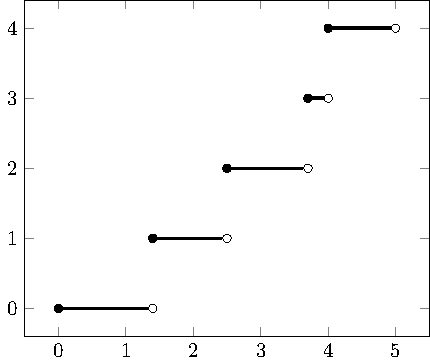
\includegraphics[width=0.5\textwidth]{figures/plots/renewal1.pdf}
\end{figure}

\item $T_i = X_i T_i'$ where  $T_i$ are i.i.d Exp$(\lambda)$ and $X_i$ i.i.d. Ber$(\frac{1}{2})$, which are independent of each other.
\begin{figure}[h]
\centering
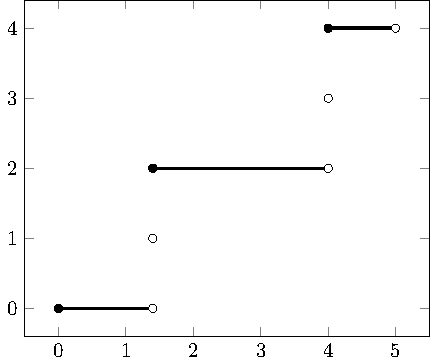
\includegraphics[width=0.5\textwidth]{figures/plots/renewal2.pdf}
\end{figure}

\item "Fat Tailed example" $\mathbb{P}_{} \left[ T_i \geq t \right] = \frac{1}{\sqrt{1+t}}\mathbbm{1}_{t\geq 0} $.
\item $T_i = 1$ a.s. the "deterministic case".
\item $T_i = \alpha $ with probability $\beta $ and $0$ with probability $1-\beta $, where $\alpha > 0$ and $0< \beta <1$. $N_t$ has law $X_0 + \sum_{i=1}^{\lfloor t/\alpha \rfloor}(1+X_i) $ where $X_i$ are i.i.d. geometric random variables with parameter  $\beta $.
	\end{enumerate}
\end{ex}

{\color{blue}
\begin{defn}
	Let $N=(N_t)_{t \geq 0}$ be a continuous time stochastic process with values in $\mathbb{R}$. We say that $N$ is a \emph{counting process} if the following holds a.s.
\begin{enumerate}
	\item $N_0 = 0$ a.s.,
	\item  $t \mapsto N_t$ is non-decreasing, right continuous, with values in $\mathbb{N}$.
\end{enumerate}
\end{defn}
}

\begin{prop}[]
	$N = (N_t)_{t\geq 0}$ is a counting process \footnote{without the condition that $N_0=0$ a.s.} with jump times $S_1, S_2, \ldots $ and $\lim_{t \to \infty} N_t = + \infty$.
\end{prop}
{\color{blue} //Is there a reason to use $+\infty$ rather than just $\infty$?. Also we have not defined a counting process at this point in time, because we are doing renewal processes before PP.//}
\begin{proof}
	Since $\mathbb{P}_{} \left[ T_i>0 \right] >0$, there exists $\alpha > 0$ such that $\mathbb{P}_{} \left[  T_i \geq \alpha  \right] >0$. Indeed $\mathbb{P}_{} \left[ T_1 >0 \right]  = \mathbb{P}_{} \left[ \bigcup_{\alpha \in \mathbb{Q}_+} \{ T_i \geq \alpha\} \right] $. We have
	\begin{align}
		\sum_{i>0}^{} \mathbb{P}_{} \left[ T_i \geq \alpha  \right] = \infty.
	\end{align}
	Therefore, by {\color{blue} the} Borel-Cantelli lemma, $\mathbb{P}_{} \left[A\right] =1$. Where
	\begin{align}
	A=	\left\{\omega: T_i(\omega) \geq \alpha \textrm{ for infinitely many } i \right\}.
	\end{align}
	For every $\omega \in A$, $S_n(\omega) \stackrel{n \to \infty}{\to} \infty$, and therefore
	\begin{align}
		t \mapsto N_t(\omega) = \sum_{n> 0}^{} \mathbbm{1}_{S_n(\omega) \leq t} 
	\end{align}
is a non-decreasing function with values in $\mathbb{N}$.	
\end{proof}


\begin{prop}[]
	There exists $c> 0$ such that
	\begin{align}
		\forall t\geq 0\ \mathbb{E}_{} \left[ e^{cN_t} \right] \leq e^{\frac{1+t}{c}}
	\end{align}
\end{prop}
\begin{rmk}[]
	In particular, for every $t \geq 1$, we have 
	\begin{align}
		\mathbb{E}_{} \left[ e^{c \frac{N_t}{t}} \right] \stackrel{\textrm(Jensen)}{\leq} \mathbb{E}_{} \left[ e^{cN_t} \right]^{\frac{1}{t}} \leq e^{\frac{2}{c}}	
	\end{align}
and
\begin{align}
	\mathbb{E}_{} \left[ \left( \frac{N_t}{t}\right)^d \right] \leq \frac{k!}{c^k}e^{\frac{2}{c}}.
\end{align}
\end{rmk}
\begin{proof}
	As before, we can pick $\alpha>0$ such that $\mathbb{P}_{} \left[ T_1 \geq \alpha  \right] >0$. For every $i> 0$, define
	\begin{align}
		T_i' = \alpha \mathbbm{1}_{T_i \geq \alpha}. 
	\end{align}
	We have $T_i' \leq T_i$ a.s. and $(T_i')$ are i.i.d. random variables with 
	\begin{align}
		T_i' = 
		\begin{cases}
			\alpha & \textrm{with probability } \beta \\
			0 & \textrm{with probability } 1-\beta
		\end{cases}
	\end{align}
	where $\beta = \mathbb{P}_{} \left[ T_1 \geq \alpha \right] > 0 $. Define $S_n'= \sum_{i=1}^{n} T_i'$ and the renewal process
	\begin{align}
		N_t' = \sum_{n> 0}^{} \mathbbm{1}_{S_n' \leq t} .
	\end{align}
	As in example {\color{blue} this example isn't here yet}, we have that
	\begin{align}
		N_t' = \stackrel{\textrm{(law)}}{=} X_0 + \sum_{i=1}^{\lfloor \frac{t}{\alpha } \rfloor} (1 + X_i),
	\end{align}
	where $(X_i)$ are geometric random variables with success parameter $\beta$. Therefore, for $c> 0$ such that $(1-\beta)e^c<1$, we have for all $t\geq 0$
	\begin{align}
	\mathbb{E}_{} \left[ e^{cN_t'} \right]  &= e ^{c\lfloor \frac{t}{\alpha}\rfloor} \prod_{i=0}^{\lfloor \frac{t}{\alpha }\rfloor} \mathbb{E}_{} \left[ e^{cX_i} \right] \\
						&\leq e^{\frac{ct}{\alpha }} \left( \frac{\beta }{1 - (1-\beta )e^c} \right)^{1 + \frac{t}{\alpha }} \\
						&\leq \left[ \left( \frac{e^c}{1 - (1-\beta )e^c} \right)^{\frac{1}{\alpha }} \right]^{1+t} \\
						&\leq e^\frac{1+t}{c}
	\end{align}
	for $c$ small enough (independent of $t$ ).
	{\color{blue} To get the second inequality, choose $\alpha \leq 1$ and use that $1+ \frac{t}{\alpha } \leq \frac{1+t}{\alpha }$ with this condition. This choice of $\alpha $ is justified as we are finding an upper bound, and $\alpha $ only appears in the denominators, thus we can choose it as small as needed.}	
\end{proof}


\begin{theorem}[Law of Large Numbers]
Write $\mu = \mathbb{E}_{} \left[ T_1 \right] $, then we have 
\begin{align}
	\lim_{t \to \infty} \frac{N_t}{t} = \frac{1}{\mu} \textrm{ a.s.}
\end{align}
\end{theorem}
\begin{rmk}[]
	If $\mu = \infty $, then $\lim_{t\to \infty } \frac{N_t}{t} = 0$ a.s.
\end{rmk}
\begin{proof}
	{\color{blue} // In your notes, you have $1/\mu $ and $\mu $ mixed up, I have made the correction here without putting it in blue, as I believe we spoke about this in the exercise class. //}

\textbf{Case 1:} $\mu < \infty $.
By the strong law of large numbers, we have 
\begin{align}
	\lim_{n \to \infty} \frac{S_{n+1}}{n+1} = \lim_{n \to \infty }\frac{S_n}{n+1} = \mu \textrm{ a.s.}
\end{align}
Notice that for every $t$ 
\begin{align}
	S_{N_t} \leq t \leq S_{N_{t}+1}.
\end{align}
Therefore,
\begin{align}
\underbrace{\frac{S_{N_t}}{N_t + 1}}_{\to \mu}
	\leq \frac{t}{N_t + 1} 
< \underbrace{\frac{S_{N_t + 1}}{N_t + 1}}_{\to \mu }.
\end{align}
Where the convergences are almost sure. Therefore $\lim_{t\to \infty } \frac{1 + N_t}{t} = \frac{1}{\mu }$ a.s., which implies that $\lim_{t \to \infty } \frac{N_t}{t} = \frac{1}{\mu} $ a.s.

\textbf{Case 2:} $\mu = \infty $.
Define $T_{i}^{(k)} = \min(k, T_i)$ for $k\geq 1$. This way we have $T_i^{(k)} \leq T_i$ a.s. and $T_i^{(k)} \uparrow T_i$ as $k \to \infty $ a.s. Consider the renewal process $N_t^{(k)}$ associated to the times $(T_i^{(k)})_{i\geq 1}$. Since $\mathbb{E}_{} \left[ T_i^{(k)} \right] \leq k < \infty$, we can apply case 1 to obtain that
\begin{align}
	\forall k \quad \lim_{t\to \infty }\frac{N_t^{(k)}}{t} = \frac{1}{\mathbb{E}_{} \left[ T_1^{(k)} \right] } \textrm{ a.s.}
\end{align}
Since $T_{i}^{(k)}\leq T_i$ a.s., we have $N_{t}^{(k)}\geq N_t$ a.s. Hence,
\begin{align}
	\forall k \quad \frac{1}{\mathbb{E}_{} \left[ T_1^{(k)} \right] } \geq \limsup_{t\to\infty} \frac{N_t}{t} \textrm{ a.s.}
\end{align}
Now, by monotone convergence, we have 
\begin{align}
	\lim_{k\to \infty } \mathbb{E}_{} \left[ T_1^{(k)} \right]  = \mathbb{E}_{} \left[ T_1 \right] = \infty,
\end{align}
and the two equations above conclude the proof.
\end{proof}

\begin{theorem}[Central Limit Theorem]
	Assume that $\mathbb{E}_{} \left[ T_1^2 \right] < \infty $. Write $\mu = \mathbb{E}_{} \left[ T_1 \right], \ \sigma^2 = Var(T_1)$. Then, assuming $\sigma>0$, we have
	\begin{align}
	\frac{N_t - \frac{t}{\mu }}{\sigma \sqrt{\frac{t}{\mu^3}}} \overset{\textrm{(law)}}{\underset{t \to \infty }{\longrightarrow}} \mathcal{N}(0,1)
	\end{align}
\end{theorem}
{\color{blue} // Proof not in notes, I believe this was an exercise, I could include that.//}

\begin{ex}[Renewal Reward Process]
	Let $(D_i)_{i\geq 1}$ be i.i.d. random variables with $D_i\geq 0$ and $\mathbb{E}_{} \left[ D_i \right] < \infty $. Define for every $t$ 
	\begin{align}
		R_t = \sum_{i\geq 1}^{} D_i \mathbbm{1}_{S_i \leq t}. 
	\end{align}
We call this the reward process, and $D_i$ the reward at time $S_i$. Then for $t $ large
\begin{align}
	\frac{R_t}{t}= \underbrace{\frac{1}{N_t} \sum_{i=1}^{N_t} D_i}_{\stackrel{\textrm{(LLN)}}{\to} \mathbb{E}_{} \left[ D_1 \right]} \underbrace{\frac{N_t}{t}}_{\to\frac{1}{\mu }}.
\end{align}
Therefore, $\frac{R_t}{t} \to \frac{\mathbb{E}_{} \left[ D_1 \right] }{\mu }$ a.s.
\end{ex}


\section{Renewal Function}
\begin{defn}
	The renewal function is defined by 
	\begin{align}
		\boxed{		\forall t\geq 0\quad  m(t) = \mathbb{E}_{} \left[ N_t \right] .}
	\end{align}
\end{defn}
\noindent
\textbf{Motivation} $m(t) = \mathbb{E}_{} \left[ \textrm{Number of points in the interval }[0,t] \right] $ where a point is a renewal time.

\begin{rmk}[]
	$m(t)<\infty$ because $N _t$ has exponential moments (Jensen).
\end{rmk}

\begin{prop}[]
	$m(t)$ is non-decreasing, non-negative, and right continuous.
\end{prop}
\begin{proof}
	We have $N_{t+s} - N_t \downarrow 0$ as $s \downarrow 0$. Therefore $m(t+s)-m(t) \to 0$ by monotone convergence. The other properties are obvious {\color{blue}\st{obvious} trivial}.
\end{proof}

\textbf{Exercise} Try to draw m(t) for the previous {\color{blue} TODO} examples.

\begin{rmk}[]
	The previous proposition implies that there exists a unique measure $\nu $ on $\mathbb{R}_+$ such that
	\begin{align}
		\forall t \quad \nu ([0,t]) = m(t).
	\end{align}
	$\nu(B)= \mathbb{E}_{} \left[ \textrm{Number of points on the set } B \right] $ for $B$ measurable.	
\end{rmk}
\noindent
\textbf{Notation} Let $G$ be a right continuous non-decreasing function on $\mathbb{R}_+$. Write $dG$ {\color{blue}for} the corresponding Lesbesgue-Stieltjes measure. For $h \in L^{1}(dG)$ or $h$ measurable and non-negative write
\begin{align}
	\int_{\mathbb{R}_+}^{} hdG = \int_{\mathbb{R}_+}^{} h(x)dG(x)
\end{align}
for the corresponding integral.

\begin{defn}[Convolution Operator]
	Let $G$ be a right continuous non-decreasing function on $\mathbb{R}_+$. Let $h: \mathbb{R}_+ \to \mathbb{R}$ {\color{blue}be} such that for all $t\geq 0$ $\int_{0}^{t} |h(t-s)|dG(s) < \infty$ or $h$ measurable non-negative. For every $t\geq 0$, define
	\begin{align}
		(h*G)(t) = \int_{0}^{t} h(t-s)dG(s).
	\end{align}
\end{defn}

\begin{rmk}[]
	If $X, Y$ are two independent random variables on $\mathbb{R}_+$ with distribution functions $F_X, F_Y$ respectively, then
	\begin{align}
		F_{X+Y} = F_X * F_Y.
	\end{align}
The proof is left as an exercise.	
\end{rmk}
\noindent
\textbf{Notation} $F^{*k} = \underbrace{F* \ldots * F}_{k \textrm{ times}}$. This is useful for the distribution function of $S_n = T_1 + \ldots + T_n$.

\begin{prop}[]
	For every $t\geq 0$ 
	\begin{align}
		m(t) = \sum_{k\geq 1}^{} F^{*k}(t).
	\end{align}
\end{prop}
\begin{proof}
	\begin{align}
		m(t) = \mathbb{E}_{} \left[ \sum_{k\geq 1}^{} \mathbbm{1}_{S_k \leq t}  \right] = \sum_{k\geq 1}^{} \mathbb{P}_{} \left[ S_k \leq t \right] = \sum_{k\geq 1}^{} F^{*k}(t).
	\end{align}
\end{proof}

\begin{theorem}[Elementary Renewal Theorem]
	\begin{align}
		\boxed{\lim_{t \to \infty} \frac{m(t)}{t}=\frac{1}{\mu }.}
	\end{align}
\end{theorem}
\begin{proof}
	We {\color{blue}already} have $\lim_{t\to \infty }\frac{N_t}{t} = \frac{1}{\mu }$ a.s. Furthermore, we have seen that $\sup_{t\geq 1} \mathbb{E}_{} \left[ \left( \frac{N_t}{t} \right)^2 \right]< \infty  $. Hence $\frac{N_t}{t}$ is uniformly integrable and 
	\begin{align}
		\lim_{t\to \infty } \frac{m(t)}{t} = \lim_{t \to \infty } \mathbb{E}_{} \left[ \frac{N_t}{t} \right]  = \mathbb{E}_{} \left[ \lim_{t \to \infty } \frac{N_t}{t} \right] = \frac{1}{\mu }.
	\end{align}
\end{proof}

\section{Renewal with Delay}
In general, the number of arrivals in $[a, a+t]$ depends on $a$, 'no stationary increments'.
\textbf{Idea} Introduce a delay. The time $\overline{T}_{1}$ is chosen with a different distribution from $\overline{T}_{2}, \overline{T}_{3}, \ldots$

We consider $(\overline{T}_{i})_{i> 0}$ independent random variables on $\mathbb{R}_+$ with
\begin{enumerate}
	\item  $\overline{T}_{1} \sim dG$,
	\item $\overline{T}_{i} \sim dF$ for $i> 1$.
\end{enumerate}
{\color{blue} TODO: Figure}
\begin{ex}[Shifted Renewal with Delay]
	$T_1, T_2, \ldots$ i.i.d. as in the previous sections. Fix $t> 0$, then define
	\begin{align}
		\overline{T}_{1} = S_{n_{t+1}}-t, \ \overline{T}_{i}= S_{N_t +i} - S_{N_t + i -1}, i> 1.
	\end{align}
\end{ex}

\begin{defn}
	\begin{align}
		\overline{S}_{i} &= \overline{T}_1 + \ldots + \overline{T}_i, \textrm{ for } i> 0\\
		\overline{N}_t &= \sum_{i> 0}^{} \mathbbm{1}_{\overline{S}_i \leq t}, \textrm{ for } t\geq 0. 
	\end{align}
	$(\overline{N}_t)_{t\geq 0}$ is called a renewal process with distribution function $F$ and delay function $G$.	
\end{defn}
\noindent
\textbf{Goal} Compute $\overline{m}(t)${\color{blue},} the renewal function associated to $\overline{N}_t$ and find $G$ such that $\overline{m}$ is linear.
\noindent
\textbf{Notation} $\overline{m}(t) = \mathbb{E}_{} \left[ \overline{N}_t \right] $. {\color{blue}// Should this be in display?//}

As in the previous section, we can prove the following
\begin{prop}[]
	\begin{align}
		\forall t\geq 0 \quad \overline{m}(t) = \sum_{i\geq 0}^{} G * F^{*i}(t).
	\end{align}
\end{prop}

The Laplace transform behaves 'nicely' with the convolution operator, and the Laplace transform of $\overline{m}$ can be easily computed.
{\color{blue}
\section{Intermezzo: Laplace Transform} 
// This is not a labeled section in your notes, but is included //}

\noindent
\textbf{Notation} $ \mathcal{M} = \{ f: \mathbb{R}_+ \to \mathbb{R}_+, \textrm{ right continuous, non-decreasing}\}$, 'non-negative measures on $\mathbb{R}_+$'. {\color{blue} $\nu((a,b])=f(b)-f(a)$ the corresponding Lebesgue-Stieltjes measure.}

\begin{defn}
	Let $f\in \mathcal{M}$. For every $s \geq 0$, define
	\begin{align}
		\boxed{ Lf(s) = \int_{0}^{\infty} e^{-sx}df(x).}
	\end{align}
\end{defn}
\begin{rmk}[]
	If $f=F_Y$ distribution function of a non-negative random variable $Y$, then $Lf(s) = \mathbb{E}_{} \left[ e^{-sY} \right] $.
\end{rmk}

\begin{prop}[]
	For every $f,g\in \mathcal{M}$, we have
	\begin{align}
		L_{f*g} = L_f \cdot L_g.
	\end{align}
\end{prop}
\begin{rmk}[]
	If $X,Y$ are two independent random variables on $\mathbb{R}_+$ then
	\begin{align}
		\mathbb{E}_{} \left[ e^{-s(X+Y)} \right] =\mathbb{E}_{} \left[ e^{-sX} \right] \mathbb{E}_{} \left[ e^{-sY} \right]. 
	\end{align}
\end{rmk}
\begin{rmk}[]
	If $f,g \in \mathcal{M}$, then $f*g$ is well defined and $f*g \in M$.
\end{rmk}
\begin{proof}
For every $h\geq 0$ measurable, we have
\begin{align}
	\int_{}^{}  h d(f*g) = \int_{}^{} \int_{}^{} h(x+y)df(x) dg(y).
\end{align}
{\color{blue} In particular, this is} true for $h=\mathbbm{1}_{(a,b]} $, because
\begin{align}
	(f*g)(b) - (f*g)(a) &= \int_{}^{} f(b-y) - f(a-y) dg(y) \\
			    &=\int_{}^{} \int_{ }^{} \mathbbm{1}_{x \in (a-y, b-y]} df(x)dg(y) \\
			    &= \int_{}^{} \int_{}^{} \mathbbm{1}_{(a,b]} (x+y) df(x)dg(y).
\end{align}
Thus, it is also true for general $h\geq 0$ by approximation. In particular for $h(x) = e^{-sx}$, we have 
\begin{align}
	\int_{}^{} e^{-sz} d(f*g)(z) = \int_{}^{} \int_{}^{} e^{-s(x+y)} df(x)dg(y) \stackrel{\textrm{(Fubini)}}{=} 
	\int_{}^{} e^{-sx}df(x) \int_{}^{} e^{-sy}dg(y).
\end{align}
\end{proof}

\begin{cor}[]
	\begin{align}
		L_{\overline{m}} = \frac{L_G}{1-L_F}.
	\end{align}
\end{cor}
\begin{proof}
	By monotone convergence, we have
	\begin{align}
		L_{\overline{m}} = \sum_{i\geq 0}^{} L_{G*F^{*i}}.
	\end{align}
	By induction $L_{G*F^{*i}}= L_{G}\cdot L_{F}^i$. Hence for all $t> 0$ (because $L_F(t) <1$) 
	\begin{align}
		L_{\overline{m}} = \sum_{i\geq 0}^{} L_{G}(t) L_{F}(t)^{i} = L_{G}(t) \sum_{i\geq 0}^{} L_{F}(t)^i= \frac{L_G(t)}{1 - L_F(t)}.
	\end{align}
This equality extends to $t=0$ since both terms are infinite.	
\end{proof}

\begin{defn}
	Consider the delay function defined by
	\begin{align}
		\forall t\geq 0 \quad G(t) = \frac{1}{\mu } \int_{0}^{t} (1-F(x))dx.
	\end{align}
\end{defn}
\begin{rmk}[]
	\begin{align}
		\int_{0}^{\infty} (1 - F(x)) dx = \int_{0}^{\infty} \mathbb{P}_{} \left[ T_1 > x \right] dx \stackrel{\textrm{(Fubini)}}{=} \mathbb{E}_{} \left[ \int_{0}^{\infty} \mathbbm{1}_{T_i > x} dx \right]  = \mathbb{E}_{} \left[ T_1 \right] = \mu .
	\end{align}
\end{rmk}

\begin{theorem}[]
	Assume $\mu <\infty$. For the renewal process with delay function $G$, we have
	\begin{align}
		\boxed{		\overline{m}(t) = \frac{t}{\mu }}
	\end{align}
	for every $t\geq 0$.
\end{theorem}
'The process is stationary.'
\begin{lemma}[]
	Let $m_1, m_2 \in \mathcal{M}$ as assume that
	\begin{align}
		\forall t>0 \quad L_{m_1}(t) = L_{m_2}(t) < \infty,
	\end{align}
Then $m_1 = m_2$.	
\end{lemma}
\begin{proof}[Proof (Lemma).]
	Admitted.
\end{proof}

\begin{proof}[Proof (Theorem).]
For $s> 0$, notice that for every $h$ measurable and bounded
\begin{align}
	\int_{0}^{\infty} h(x)dG(x) = \int_{0}^{\infty} h(x)(1-F(x)) \frac{dx}{\mu }. 
\end{align}
This is done as usual, first showing for $h=\mathbbm{1}_{[a,b]} $ and then concluding by approximation.
In particular, for every $s> 0$ 
\begin{align}
	L_G(s) &\stackrel{\phantom{\textrm{(Fubini)}}}{=}  \int_{0}^{\infty} e^{-sx}dG(x) = \int_{0}^{\infty} e^{-sx}\underbrace{(1-F(x))}_{=\mathbb{P}_{} \left[ \overline{T}_2>x \right] } \frac{dx}{\mu } \\
	       &\stackrel{\phantom{\textrm{(Fubini)}}}{=}  \frac{1}{\mu s} \int_{0}^{\infty} s e^{-sx} \mathbb{P}_{} \left[ \overline{T}_2>x \right] dx \\
	       &\stackrel{\textrm{(Fubini)}}{=} \frac{1}{s \mu } \mathbb{E}_{} \left[ \int_{0}^{\infty} s e^{-sx}\mathbbm{1}_{\overline{T}_2>x} dx \right]  \\
	       &\stackrel{\phantom{\textrm{(Fubini)}}}{=}  \frac{1}{s \mu } \mathbb{E}_{ } \left[ \int_{0}^{\overline{T}_2} s e^{-sx}dx \right] \\
	       & \stackrel{\phantom{\textrm{(Fubini)}}}{=} \frac{1}{s \mu } \mathbb{E}_{} \left[ 1 - e^{-s \overline{T}_2} \right]  = \frac{1-L_F(s)}{s\mu }.
\end{align}
Therefore
\begin{align}
	L_{\overline{m}}(s) &= \frac{1-L_F(s)}{s\mu }\frac{1}{1-L_F(s)} =  \frac{1}{s\mu } \\
			    &= \frac{1}{\mu } \int_{0}^{\infty} e^{-sx}dx = L_{\frac{1}{\mu }I}.
\end{align}
Where $I$ is the identity function. By the lemma, we conclude that for all $t\geq 0$ $\overline{m}(t) = \frac{1}{\mu }t$.
\end{proof}


\section{Blackwell's Renewal Theorem}
\begin{defn}
	We say that the law of $T_1$ is \emph{non-arithmetic} if
	\begin{align}
		\forall a> 0 \quad \mathbb{P}_{} \left[ T_1 \in a \mathbb{Z} \right] < 1.
	\end{align}
	
\end{defn}

{\color{blue}
\begin{defn}
	We say the law of $T_1$ is \emph{arithmetic} if there exists $a > 0$ such that 
\begin{align}
	\mathbb{P}_{} \left[ T_1 \in a \mathbb{Z} \right] =1.
\end{align}
	It is \emph{non-arithmetic} if this probability is $<1$.
\end{defn}
}

\begin{theorem}[Blackwell's Renewal Theorem]
	Assume that the law of $T_1$ is non-arithmetic, then for all $h\geq 0$
	\begin{align}
	\boxed{ \lim_{t \to \infty} m(t+h)-m(t) = \frac{h}{\mu }.}
	\end{align}
	
\end{theorem}

{\color{blue} // This is from your lecture, but not in the notes.//
\begin{rmk}[]
	\begin{align}
		 \frac{m(t)}{t} \approx \frac{m(\lfloor t \rfloor)}{\lfloor t \rfloor} = \frac{1}{\lfloor t \rfloor} \sum_{k=1}^{\lfloor t \rfloor} m(k) - m(k-1) \stackrel{\textrm{(Blackwell)}}{\to} \frac{1}{\mu}. 
	\end{align}
	"Blackwell is stronger than elementary renewal."
\end{rmk} }

\begin{proof}[Proof (Sketch)]
	Consider $\overline{T}_i,\ i> 0$ independent and independent of $(T_i)_{i> 0}$ where $\overline{T}_1$ has law $dG$, and $\overline{T}_{i}$ has law $dF$ for $i> 1$.
	Then the renewal function associated to these inter-arrival times is
	\begin{align}
		\forall t \quad \overline{m}(t) = \frac{1}{\mu }t.
	\end{align}
We call this 'stationary'. Write $S_k = \sum_{i\leq k}^{} T_i$ and $\overline{S}_k = \sum_{i \leq k}^{} \overline{T}_i$.

Now claim that for $\epsilon > 0$, a.s. there exists $K>1$ (random) such that
\begin{align}
|S_K - \overline{S}_K | \leq \epsilon.
\end{align}
We admit this.

\begin{figure}[h]
	\centering
	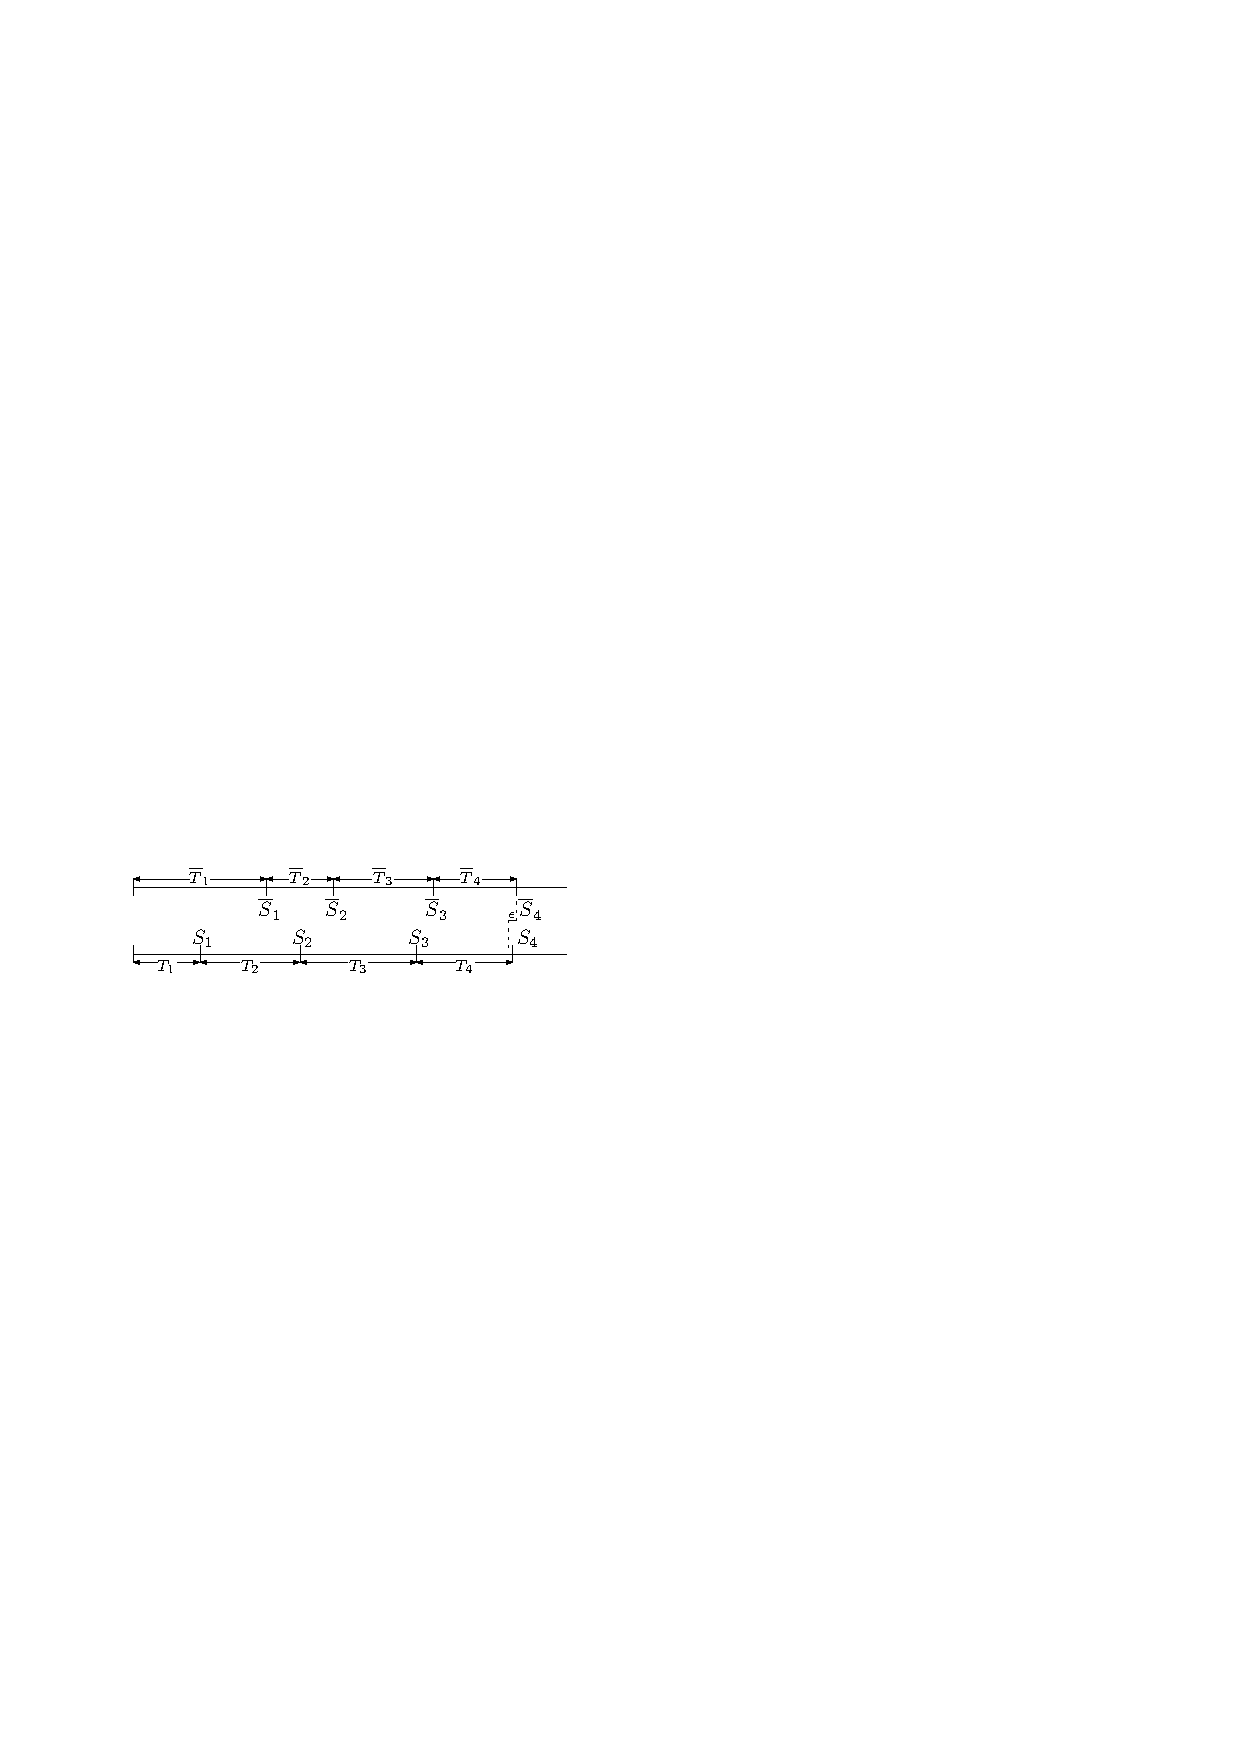
\includegraphics[width=0.6\textwidth]{figures/blackwell.pdf}
	\caption{Example of such a $K$, here $K=4$.}
\end{figure}


Consider 
\begin{align}
	\tilde{T}_i =
	\begin{cases}
		\overline{T}_i, & i \leq k \\
		T_i, & i>K.
	\end{cases}
\end{align}
Then the renewal process associated to $(\tilde(T)_i)_{i>0}$ is a delayed process with renewal function
\begin{align}
	\tilde{m}(t) = \frac{t}{\mu }.
\end{align}
Furthermore for $t$ large ($t>K$), we have
\begin{align}
	N_{t+h} - N_t \approx \tilde{N}_{t+h} - \tilde{N}_{t}.
\end{align}
Therefore
\begin{align}
	m(t+h) - m(t) = \mathbb{E}_{} \left[ N_{t+h} - N_t \right] \approx \mathbb{E}_{} \left[ \tilde{N}_{t+h} - \tilde{N}_{t} \right] = \frac{h}{\mu }.
\end{align}
\end{proof}

\section{Renewal Equation}

\begin{defn}
	Let $h:\mathbb{R}_+ \to \mathbb{R}$ be measurable locally bounded, $g:\mathbb{R}_+ \to \mathbb{R}$ such that for all $t\geq 0$ $\int_{0}^{t} |g(t-s)|dF(s) <\infty$. We say that $g$ is a solution of the $(h,F)$ renewal equation if
\begin{align}
	\boxed{ \forall t\geq 0 \quad g(t) = h(t) + \int_{0}^{t} g(t-s)dF(s) ,}
\end{align}
ie. $g=h+g*F$.
\end{defn}

\begin{prop}[]
	$m$ is a solution of the $(F,F)$ renewal equation, ie. $m=F+m*F$.	
\end{prop}
\begin{proof}[Proof 1]
\begin{align}
	m = \sum_{i> 0}^{} F^{*i} = F + \sum_{i> 1}^{} F^{*(i-1)}*F = F + \underbrace{\left( \sum_{i> 1}^{} F^{*(i-1)} \right)}_{m}*F.
\end{align}
\end{proof}
\begin{proof}[Proof 2]
For $t\geq 0$, we have
\begin{align}
	m(t)& = \mathbb{E}_{} \left[ \sum_{k> 0}^{} \mathbbm{1}_{T_1 + \ldots + T_k \leq t}  \right] = \mathbb{P}_{} \left[ T_1 \leq t \right] + \underbrace{\mathbb{E}_{} \left[ \sum_{k> 1}^{}\mathbbm{1}_{T_1 + \ldots + T_k \leq t}   \right]}_{(\star)} \\ 
	(\star) &\stackrel{\textrm{(Fubini)}}{=} \sum_{k> 1}^{} \mathbb{E}_{} \left[ \mathbbm{1}_{T_1 + \ldots + T_k \leq t}  \right] \stackrel{\textrm{(Indep.)}}{=} \sum_{k> 1}^{} \int_{0}^{t} \mathbb{E}_{} \left[ \mathbbm{1}_{s+T_2+\ldots+T_k \leq t}  \right] dF(s) \\
		&\stackrel{\textrm{\phantom{(Fubini)}}}{=} \int_{0}^{t} m(t-s)dF(s).
\end{align}
\end{proof}

\begin{ex}[Generalization]
	Let $E= \{ (s_i)_{i> 0}: s_1 \leq s_2\leq \ldots,\ s_{i}\to \infty\} \subset \mathbb{R}^{\mathbb{N}}$, where $\mathbb{R}^{\mathbb{N}}$ is equipped with the product $\sigma$-algebra.
	Let $\Phi:E \to \mathbb{R}$ be measurable such that
	\begin{align}
		\forall t\geq 0,\ i=1,2 \quad \mathbb{E}_{} \left[ | \Phi(S_i-t, S_{i+1}-t,\ldots)| \right] < \infty.
	\end{align}
	Define $\phi(t)=\mathbb{E}_{} \left[ \Phi(S_1-t, S_2-t,\ldots)] \right] $ for all $t\geq 0$.	
\end{ex}
{\color{blue} // TODO: Possible figure? //}

\begin{prop}[]
	$\phi$ is a solution of the $ (h,F)$ renewal equation, where for all $t\geq 0$
	\begin{align}
		h(t) = \mathbb{E}_{} \left[ \Phi(S_1 -t, S_2-t, \ldots) \right] - \mathbb{E}_{} \left[ \Phi(S_2 - t, S_3-t, \ldots)\mathbbm{1}_{T_1\leq t}  \right] ,	
	\end{align}
	ie. for all $t\geq 0$ $\phi(t) = h(t) + \int_{0}^{t} h(t-s)dF(s)$.
\end{prop}

\begin{proof}
	\begin{align}
		\mathbb{E}_{} \left[ \Phi(S_1 - t, S_2-t, \ldots) \right] 
		&= h(t) + \mathbb{E}_{} \left[ \Phi(S_2 -t, S_3-t,\ldots)\mathbbm{1}_{T_1 \leq t}  \right] \\
		&= h(t) + \mathbb{E}_{} \left[ \Phi(T_1 + T_2 - t, T_1+T)2 + T_3 -t, \ldots)\mathbbm{1}_{T_1\leq t}\right] \\ 
		&= h(t) + \int_{0}^{t} \mathbb{E}_{} \left[ \Phi(s+T_2 -t, s+T_2+T_3-t,\ldots) \right] dF(s) \\
		&= h(t) + \int_{0}^{t} \phi(t-s)dF(s).
	\end{align}
\end{proof}

\begin{ex}[Application 1]
	$m$ is a solution of the $(F,F)$ renewal equation. {\color{blue}To use this, we have to bring it into the proper form.} $N_t = \Phi(S_1-t, S_2-t,\ldots)$ where $\Phi(s_1,s_2,\ldots) = \sum_{i}^{} \mathbbm{1}_{s_i\leq 0} $. Hence, $m(t) = \mathbb{E}_{} \left[ N_t \right]$ is the solution of the $(h,F)$ renewal equation with
	\begin{align}
		h(t) = \mathbb{E}_{} \underbrace{\left[ \Phi(S_1-t, S_2-t,\ldots) - \mathbbm{1}_{T_1\leq t} \Phi(S_2-t, S_3-t, \ldots)  \right]}_{=
	\begin{cases}
		0, &T_1>t \\
		1, &T_1\leq t
	\end{cases}
}
	\end{align}
	ie. $h(t) = \mathbb{P}_{} \left[ T_1 \leq t \right] $.	
\end{ex}

\begin{ex}[Application 2]
	For $t\geq 0$, define $E_t = S_{N_{t+1}}-t${\color{blue}, the time left to wait until next renewal}. Define for  $x \geq 0$, $e_x(t) = \mathbb{P}_{} \left[ E_t \leq x \right] $ for all $t\geq 0$. 

	{\color{blue} First we will find a solution without the proposition. We can separate $e_x$ into two parts, one for the probability if there has already been a renewal before time $t$, and one if that hasn't occurred $e_x(t) = \mathbb{P}_{} \left[ T_1 > t, E_t \leq x \right]  + \mathbb{P}_{} \left[ T_1 \leq t, E_t \leq x \right]  = A + B$.
\begin{align}
	A = \mathbb{P}_{} \left[ T_1 > t, T_1 \leq t+x \right] = F(t+x)-F(t).
\end{align}
Observe that $E_t$ is measurable with respect to $(T_1, T_2, \ldots)$. Write $\phi_t(T_1,T_2, \ldots )=E_t$. 
\begin{align}
	\mathbb{P}_{} \left[ T_1 \leq t, E_t \leq x \right] =& \mathbb{P}_{} \left[ T_1 \leq t, \phi_t(T_1,T_2, \ldots ) \leq x \right] \\ 
	=& \int_{0}^{t} \mathbb{P}_{} \left[ \phi_t(s, T_2, \ldots ) \leq x \right] dF(s) = \int_{0}^{t} \mathbb{P}_{} \left[ E_{t-s} \leq x \right] dF(s) \\
	=& \int_{0}^{t} e_x(t-s) dF(s) = (e_x * F)(t)
\end{align}
Thus $e_x(t) = h_x(t) + (e_x * F)(t)$ with $h_x(t) = F(t+x)-F(t)$. So  $e_x$ is a solution of the $(h_x,F)$ renewal equation.
}

{\color{blue}To use the proposition, we have to bring our problem into the correct form. }We have that $e_x(t) = \mathbb{E}_{} \left[ \Phi(S_1-t, S_2-t,\ldots) \right] $ where $\Phi(s_1, s_2,\ldots) = \mathbbm{1}_{\min\{s_i:\ s_i\geq 0\}\leq x}$. Then $e_x$ is a solution of the $(h,F)$ renewal equation, where
\begin{align}
h(t) &= \mathbb{E}_{} \underbrace{\left[ \Phi(S_1 -t,\ldots) - \mathbbm{1}_{T_1\leq t}\Phi(S_2-t,\ldots) \right] }_{=
\begin{cases}
	0, &T_1\leq t \textrm{ or } T_1>t+x \\
	1, & t<T_1\leq t+x
\end{cases}
} \\
&= \mathbb{P}_{} \left[ t<T_1 \leq t+x \right] = F(t+x)-F(t).
\end{align}

\end{ex}

\section{Well-Posedness of the Renewal Equation}
\begin{theorem}[]
	Let $h: \mathbb{R}_+\to \mathbb{R}$ be measurable, locally bounded. Then there exists a unique $g: \mathbb{R}_+ \to \mathbb{R}$ measurable, locally bounded, and a solution of $g = h + g*F$ is given by $g=h+h*m$. 
\end{theorem}
{\color{blue}
\begin{proof}[Intuitive Proof]
	This is only to show how to get the idea that $g=h+h*m$ is a solution. Assume $g$ is a solution, then we have 
\begin{align}
	g =& h + g*F \\
	=& h + (h+g*F)*F \\
	 \vdots  \\
	\stackrel{(*)}{=}& h + h*F + h*F^{*2} + h*F^{*3}+ \ldots  \\
	=& h + h*m
\end{align}
\end{proof}
}
\begin{proof}[Rigorous Proof]
	\textbf{Existence} 
	$g = h + h*m$ is measurable and locally bounded, because $h$ is. We have 
	\begin{align}
		h + g*F &= h + (h+h*m)*F \\
			&= h + h*\underbrace{(F+m*F)}_{=m}= g.
	\end{align}

\textbf{Uniqueness} 
Let $g_1, g_2$ be two solutions of the $(h,F)$ renewal equation. Then $g_1-g_2 = (g_1 - g_2)*F = (g_1 - g_2) * F^{*n}$. We have for every $t \geq 0$
\begin{align}
	 |g_1(t) - g_2(t)| = \left| \int_{0}^{t} (g_1 - g_2)(t-s)dF^{*n}(s) \right| \leq \sup_{[0,t]} |g_1 - g_2| \int_{0}^{t} dF^{*n}(s).
\end{align}
Where we can see the integral term is equal to $\mathbb{P}_{} \left[ T_1 + \ldots  +T_n \leq t \right] $ which converges to 0. Hence $g_1 = g_2$.
\end{proof}

\section{Asymptotic Behavior}
In this section we assume that the law of $T_1$ is non-arithmetic.

\noindent
\textbf{Motivation} Let $g$ be the solution of the $(h,F)$ renewal equation, what is the asymptotic behavior of $g(t)$ for $t\to \infty$?

\noindent
\textbf{Case 1} $h=\mathbbm{1}_{[a,b]} $ for $0\leq a \leq b$ and $g$ the solution of the $(h,F)$ renewal equation. 
\begin{align}
	g(t) &= h(t) + \int_{0}^{t} h(t-s)dm(s) = h(t) + \int_{t-b}^{t-a} h(s)dm(s) \\
	     &= \underbrace{h(t)}_{\to 0} + \underbrace{m(t-a) - m(t-b)}_{\stackrel{\textrm{(Blackwell)}}{\to} \frac{b-a}{\mu }}.
\end{align}
Where it was assumed that $t$ was large in the last two equalities. Hence $\lim_{t\to \infty } g(t) \frac{1}{\mu } \int_{0}^{\infty} h(s) ds$. 

\noindent \textbf{Question} How does this generalize?

{\color{blue}\noindent
\textbf{Idea} Extend to simple functions $\sum_{}^{} \lambda_i \mathbbm{1}_{I_i}$ (this is easy), then try to extend to directly integrable Riemann functions.}

\begin{defn}
	$h: \mathbb{R}_+ \to \mathbb{R}_+$ measurable, $h$ is called \emph{directly Riemann Integrable} (dRi) if 
\begin{align}
	\forall \Delta >0 \quad \sum_{k=0}^{\infty}\Delta \sup_{[k \Delta, (k+1)\Delta]} h < \infty
\end{align}
	and
	\begin{align}
		\lim_{\Delta \to 0} \Delta \sum_{k=0}^{\infty} \sup_{[k \Delta,(k+1)\Delta] } h = \lim _{\Delta \to \infty} \Delta \sum_{k=0}^{\infty} \inf_{[k \Delta, (k+1)\Delta]}h.
	\end{align}
	$h: \mathbb{R}_+ \to \mathbb{R}_+$ is dRi if and only if $h_+=\max(h,0)$ and $h_-=\max(-h,0)$ are dRi.
\end{defn}
\begin{rmk}[Counter Example]
	$h=\sum_{k> 0 }^{} \mathbbm{1}_{[k,k+2^{-k}]} $ is integrable, but is not dRi.	
\begin{figure}
	\centering
\begin{tikzpicture}
	\begin{axis}[xmin=0, xmax=4.5, ymin=0, ymax=1.2]
		\addplot[samples=20, black] coordinates{(1,0) (1,1) (1.5,1) (1.5,0) (2,0) (2,1) (2.25,1)
			(2.25,0) (3,0) (3,1) (3.125, 1) (3.125, 0) (4,0) (4,1) (4.0625, 1) (4.0625, 0)};	
	\end{axis}
\end{tikzpicture}
\end{figure}
\end{rmk}


\begin{prop}[]
	Let $h: \mathbb{R}_+ \to \mathbb{R}$ be measurable. Assume that $h$ is continuous at a.e. $t \in \mathbb{R}$ and there exists $H$ non-decreasing such that $0 \leq |h| \leq H$ and $\int_{0}^{\infty} H < \infty$. Then $h$ is dRi. 
\end{prop}
\begin{rmk}[]
	In particular if $h$ is bounded, continuous at a.e. $t \in \mathbb{R}$, and vanishes outside a compact set, the $h$ is dRi.
\end{rmk}
{\color{blue}// The proof is omitted and given in Sznitman's notes, I think we should include it here.//}

\begin{theorem}[Smith Key Renewall Theorem]
	Let $h$ be dRi, $F$ non-arithmetic. Then $g=h+h*m$ satisfies 
\begin{align}
\boxed{\lim_{t \to \infty}g(t)= \frac{1}{\mu } \int_{0}^{\infty} h(u) du.}
\end{align}
\end{theorem}

\begin{rmk}[]
	The case $h= \mathbbm{1}_{[0,b]}$ corresponds to the Blackwell Theorem. 
\end{rmk}

{\color{blue}The idea of the proof is to use an approximation of $h$ by functions of the form $h_{c,\Delta}=\sum_{k\geq 0}^{} c_k \mathbbm{1} _{[k\Delta, (k+1)\Delta)}$.}

\begin{proof}
	since $h$ is dRi we have
	\begin{align}
		\sum_{k}^{} \sup_{[k,k+1]}h<\infty.
	\end{align}
	Hence $h(t) \to 0$. Therefore it suffices to prove
	\begin{align}
		\lim_{t\to \infty} \int_{0}^{t} h(t-s)dm(s) = \frac{1}{\mu }\int_{0}^{t} h(u)du.
	\end{align}
	Let $\Delta>0$ such that $F(\Delta) < 1$. 

	Assume $h = \sum_{k\geq 0}^{} c_k \mathbbm{1}_{[k\Delta, (k+1)\Delta)} $ with  $c_k\geq 0$ and $\sum_{k\geq 0}^{} c_k < \infty$. By monotone convergece
	\begin{align}
		h(t-s)dm(s) = \sum_{k\geq 0}^{} \underbrace{c_k [m(t - k\Delta) - m(t-k\Delta - \Delta)]}_{h_{k}(t)}.
	\end{align}
Observe that for every $u\geq \Delta$
 \begin{align}
	 1 \geq F(u) &= m(u) - \int_{0}^{u} F(u-s)dm(s) = \int_{0}^{u} (1-F(u-s))dm(s) \\
		     &\geq \int_{u-\Delta}^{u} (\underbrace{1-F(u-s)}_{\geq1-F(\Delta)}) dm(s) \geq \left(1-F(\Delta)\right)\left(m(u) - m(u-\Delta)\right). 
\end{align}
In the first equality, it was used that $m$ is the solution of the $(F,F)$ renewal equation. Hence for every $t$ and every $k$ 
\begin{align}
	h_k(t) \leq \frac{c_k}{1-F(\Delta)},
\end{align}
by distinguishing between $t-k\Delta \geq \Delta$ and $t-k\Delta<\Delta$, and using that $m$ is non-decreasing, vanishing on $(-\infty, 0)$.
By dominated convergence
\begin{align}
	\lim_{t\to \infty} \sum_{k\geq 0}^{} h_k(t) = \sum_{k\geq 0}^{} \underbrace{\lim_{t\to \infty} h_k(t)}_{\stackrel{\textrm{(Blackwell)}}{=} c_k \frac{\Delta}{\mu }}.
\end{align}
Hence $\lim_{t\to \infty} \int_{0}^{t} h(t-s)dm(s) = \sum_{k=0}^{\infty} c_k \frac{\Delta}{\mu } = \frac{1}{\mu }\int_{0}^{\infty} h(u)du.$ 

Now assume $h\geq 0$ dRi. Let $\Delta>0$ such that $F(\Delta)<1$. Write
\begin{align}
	\underline{h}_{\Delta} &= \sum_{k\geq 0}^{} (\inf_{[k\Delta, (k+1)\Delta]}h) \mathbbm{1}_{[k\Delta, (k+1)\Delta)} \\
	\overline{h}_{\Delta} &=  \sum_{k\geq 0}^{} (\sup_{[k\Delta, (k+1)\Delta]}h) \mathbbm{1}_{[k\Delta, (k+1)\Delta)}. 
\end{align}
We have for every $t$ 
\begin{align}
	\int_{0}^{t} h(t-s)dm(s) \leq \int_{0}^{t} \overline{h}_{\Delta}(t-s) dm(s) \to  \frac{1}{\mu }\int_{0}^{t} \overline{h}_{\Delta}(u)du.
\end{align}
Hence
\begin{align}
	\limsup_{t\to\infty} \int_{0}^{t} h(t-s)dm(s) \leq \frac{1}{\mu }\int_{\mathbb{R}}^{} \overline{h}_{\Delta}(u)du.
\end{align}
Since
\begin{align}
	\left| \int_{\mathbb{R}}^{} \overline{h}_{\Delta}(u) du - \int_{\mathbb{R}}^{} h(u) du \right| \leq \sum_{k\geq 0}^{} \Delta \left(\overline{h}_{\Delta}(k\Delta) - \underline{h}_{\Delta}(k\Delta)\right) \stackrel{\Delta\to0}{\longrightarrow} 0,
\end{align}
where the limit is due to $h$ being dRi. We can let $\Delta$ tend to 0 in the equation above {\color{blue}(with $\limsup$)} to obtain
\begin{align}
	\limsup_{t\to\infty} \int_{0}^{t} h(t-s)dm(s) \leq \frac{1}{\mu }\int_{\mathbb{R}}^{} h(u)du,
\end{align}
and equivalently
\begin{align}
	\liminf_{t\to\infty} \int_{0}^{t} h(t-s)dm(s) \geq \frac{1}{\mu }\int_{\mathbb{R}}^{} h(u)du.
\end{align}
{\color{blue}
\begin{align}
	\frac{1}{\mu }\int_{\mathbb{R}}^{} h(u)du \leq \liminf_{t\to\infty} \int_{0}^{t} h(t-s)dm(s) 
	\leq
	\limsup_{t\to\infty} \int_{0}^{t} h(t-s)dm(s) \leq \frac{1}{\mu }\int_{\mathbb{R}}^{} h(u)du.
\end{align}
}
\end{proof}

{\color{blue}
// This was done in class //

\noindent \textbf{Application} Let $\mu < \infty$. Let $E_t$ be the excess time (time until next renewal) and $e_x(t) = \mathbb{P}_{} \left[ E_t \leq x \right] $. What is $\lim_{t \to \infty} e_x(t)$? We know that $e_x = h_x + e_x*F$, where $h_x(t) = F(t+x)-F(t)$.
\begin{rmk}[]
	$\mu = \mathbb{E}_{} \left[ T_1 \right] = \int_{0}^{\infty} \mathbb{P}_{} \left[ T_1 > t \right] dt$
\end{rmk}
\noindent With this we have that $h_x(t) \leq 1 - F(t) = \mathbb{P}_{} \left[ T_1 > t \right] $, and $1-F(t)$ is non-increasing in $t$ and continuous a.e. (because it is the difference of two monotone functions). 
\begin{align}
	\int_{0}^{\infty} \mathbb{P}_{} \left[ T_1 > t \right] dt = \mathbb{E}_{} \left[ T_1 \right] = \mu < \infty .
\end{align}
Thus (by the proposition) $h_x$ is dRi. Now we can apply the theorem and get that 
\begin{align}
	\lim_{t \to \infty} \mathbb{P}_{} \left[ E_t \leq x \right] = \frac{1}{\mu } \int_{0}^{\infty} h_x(t)dt = \frac{1}{\mu } \int_{0}^{\infty} F(t+x) - F(t) dt,
\end{align}
with $F(t+x) - F(t) = \mathbb{E}_{} \left[ \mathbbm{1}_{T_1 \in (t, t+x]} \right] $, we find that the limit is equal to 
\begin{align}
	\frac{1}{\mu } \int_{0}^{\infty} \mathbb{E}_{} \left[ \mathbbm{1}_{T_1 \in (t, t+x]} \right]dt = \frac{1}{\mu} \mathbb{E}_{} \left[ \int_{0}^{ \infty } \mathbbm{1}_{t \in [T_1 -x, T_1)}    \right]dt = \frac{1}{\mu } \mathbb{E}_{} \left[ \int_{\max\{T_1-x, 0\}}^{T_1} dt \right] =  
	\begin{cases}
		T_1, & T_1 \leq x \\
		x, & T_1 > x.
	\end{cases}
\end{align}
Thus for $t$ large:  $\mathbb{P}_{} \left[ E_t \leq x \right] \approx  \frac{1}{\mu} \mathbb{E}_{} \left[ \min\{T_1, x\} \right]  $. 

\begin{rmk}[]
	$G(x) = \frac{1}{\mu } \mathbb{E}_{} \left[ \min\{T_1, x\} \right] $ is the delay distribution in the proof of Blackwell's Theorem.
\end{rmk}
}
\noindent \textbf{Conclusion} We have now used renewal processes to define a general structure to model a real life process mathematically. Using this object enabled us to implement the LLN and make statements about the asymptotic behavior of such processes over large periods of time.



\newpage

\chapter{General Poisson Point Processes}
\textbf{Reference} Lectures on the Poisson Process (Penrose), Poisson Processes (Kingman)

\section{Introduction}
\textbf{Question} How can we represent points on $\mathbb{R}_+$ mathematically?
\begin{enumerate}
	\item A set of points $\mathcal{S}=\{S_1, S_2,...\}$ \label{q:3}
	\item 'Time point of view', ie $T_1,T_2,...$ where $T_i$ = time between the $(i-1) $'th and $i $'th point. \label{q:1}
	\item Cadlag formulation with values in $ \mathbb{N}$. $N_t=$ number of points in $[0,t]$. \label{q:2}
	\item Measure $N: \mathcal{B}(\mathbb{R}_+) \to \mathbb{N}$ with $N(A)=$ number of points in $A$. \label{q:4}
\end{enumerate}
\textbf{Goal} Define $\Omega \to $'set of points'. For a general state space $\mathbb{R}^2, [0,1]^2,$ a manifold, etc. 
\ref{q:1} and \ref{q:2} are specific to $\mathbb{R}_+$, so they do not generalize. \ref{q:3} is not very easy to describe. \ref{q:4} is actually nice, so we will  use this point of view.

\textbf{Framework} $(E,d)$ a Polish space (separable, complete, metric space). $\mathcal{E}$ Borel $\sigma$-algebra. $\mu: \sigma$ finite measure on $(E, \mathcal{E})$, ie  $\exists  B_i \uparrow E: \mu(B_i)<\infty$ where $B_i \uparrow E \iff B_1 \subset B_2 \subset...: \bigcup_{i\geq 1}B_i=E$.

\begin{ex}[] Of such spaces: 
\begin{enumerate}
	\item $E=\{0\}, \mu = \delta_0$
	\item $E=\mathbb{R}_+, \mu = \lambda \mathcal{L}$
	\item $E=\mathbb{R}^2, \mu(dx)=\frac{1}{\pi} e^{- |x|^2}dx$ 'Gaussian'
\end{enumerate}
\end{ex}

\textbf{Goal} We wish to define a point process on $(E, \mathcal{E})$ where the 'number of points around $x$ ' $\approx \mu(dx)$ on $\mathbb{R}_+$. 

\section{Point Processes}
\textbf{Notation} $\mathcal{N}=\{\nu: \nu=\sigma-$finite measure st $\forall B \in \mathcal{E}: \nu(B) \in \mathbb{N} \cup \{+\infty\}\}$.
\noindent
\textbf{Measure Structure} Let $\mathcal{B}(\mathcal{N})$ be the $\sigma$-algebra generated by the sets $\{\nu \in \mathcal{N}: \nu(B)=k\}=\mathcal{N}_k$ for $B \subset E$ meas and $k \in \mathbb{N}$. $\to (\mathcal{N}, \mathcal{B}(\mathcal{N}))$ measured space.

\begin{prop}[]
	Let $\mathcal{N}_{<\infty}=\{\nu \in \mathcal{N}: \nu(E)<\infty \}$, there exists meas maps $\tau: \mathcal{N}_{< \infty} \to \mathbb{N}, X_i: \mathcal{N}_{< \infty} \to E$ st $\forall \nu \in \mathcal{N}_{<\infty}: \nu = \sum_{i=0}^{\tau(\nu)} \delta_{X_i(\nu)}$.
\end{prop}

\begin{defn}
	A point process on $(E, \mathcal{E})$ is a RV $N$ with values in $ \mathcal{N}$. '$N$ is a random $\sigma$-finite measure', $N \leftrightarrow$ 'random set of points'. 
\end{defn}
This means $N: \Omega \to \mathcal{N} $ meas, for any fixed $B \subset E: N(B): \Omega \to \mathbb{N}\cup \{+\infty\}$ is measurable. 
Thus a stochastic process corresponds to $(N(B))_{B \in \mathcal{E}}$. '$N(B)=$ number of points in B'.

\begin{ex}[] Point Processes:
\begin{itemize}
	\item $N=0$ a.s.  $\to$ empty set
	\item $E=[0,1], X$ RV on  $[0,1]$.  $N=\delta_X$ is a point process.
	\item $X_1,...X_n$ iid RV on $[0,1]$,  $N=\delta_{X_1}+...+\delta_{X_n}$ is a point process.
\end{itemize}
\end{ex}

\section{Poisson Point Processes}
\textbf{Setup} $(E, \mathcal{E})$ Polish, $\mu$ fixed $\sigma$-finite measure (think of $\lambda \mathcal{L}$ ), $ \mathcal{N}=\{\sigma$ finite counting measure$\}$, $(\Omega, F, \mathbb{P} )$ abstract prob space.

\begin{defn}
	A Poisson process with intensity $\mu$ on $(E, \mathcal{E})$ ($ppp(\mu)$) is a point process st:
 \begin{enumerate}
	 \item $\forall B_1...B_k \subset E$ meas and disjoint: $N(B_1)...N(B_k)$ are indep.
	 \item $\forall B \subset E$ meas $N(B) \sim Pois(\mu(B))$.
\end{enumerate}
\end{defn}

\section{Existence and Uniqueness}
\textbf{Question} Does there always exist a $ppp(\mu)$ on $E$?
\subsubsection{Spaces with finite measure}
\begin{prop}[]
	Let $Z \sim Pois(\mu(E))$, $(X_i)_{i\geq 1}$ iid where $X_i \sim \frac{\mu(.)}{\mu(E)}$. Then $N= \sum_{i=1}^{Z} \delta_{X_i} $ is a $ppp(\mu)$ on $E$.
\end{prop}

\subsubsection{Superposition}
\begin{lemma}[]
	Let $\lambda = \sum_{i=1}^{\infty} \lambda_i, \lambda_i\geq 0$. $X_i \sim Pois(\lambda_i), i \geq 1$ indep, then $X = \sum_{i=1}^{\infty} X_i \sim Pois(\lambda)$.
\end{lemma}

\begin{theorem}[]
	Let $N_i, i\geq 1$ be a sequence of indep $ppp(\mu_i)$ where $\mu_i$ and $\mu = \sum_{i=1}^{\infty} \mu_i$ are $\sigma$-finite measures. Then $N= \sum_{i=1}^{\infty} N_i$ is a $ppp(\mu )$.
\end{theorem}

\begin{cor}[]
	$\mu \ \sigma$-finite measure on $(E, \mathcal{E})$, then $\exists\ ppp(\mu)$ on $E$.
\end{cor}

\subsubsection{Uniqueness}
Let $N$ be a $ppp(\mu )$ on $E$, define $P_N = $ law of $N$ ($\rightarrow$ a probability meas on $ \mathcal{N}$).

\begin{prop}[]
	Let $N, N'$ be two $ppp(\mu )$ on $(E, \mathcal{E})$ then $P_N = P_{N'}$.
\end{prop}

\begin{theorem}[Representation of ppp as Proper Processes]
	Let $N$ be a $ppp(\mu )$ on $(E, \mathcal{E})$, there exists some RV $\tau \in \mathbb{N} \cup \{+\infty \}$ st: $X_n \in E, n\geq 1: N = \sum_{i=1}^{\tau(} $
\end{theorem}

\section{Laplace Functional}
$N$ a random meas on $(E, \mathcal{E})$ for $u:E \to \mathbb{R}$ what should we interpret $\int_E u dN$ as?

\begin{lemma}[]
	$X \sim Pois(\lambda ), \lambda > 0$, then $\forall u\geq 0: \mathbb{E}_{} \left[ e^{-u X} \right] = exp( - \lambda (1 - e^{-u}))$.
\end{lemma}

\begin{defn}
	Let $N$ be a point process on $(E, \mathcal{E})$, for every $u:E\to \mathbb{R}_+$ define $L_N(u) = \mathbb{E}_{} \left[ exp(- \int u(x) N(dx) \right] $
\end{defn}

\begin{rmk}[]
	$\int_E u(x) N(dx) = \int_E u dN$ is a RV.
\end{rmk}

\begin{theorem}[Characterization via Laplace Functional]
	Let $\mu \ \sigma$-finite meas on $(E, \mathcal{E})$. Let $N$ be a point process on $E$. TFAE:
\begin{enumerate}
	\item $N$ is a $ppp(\mu)$ 
	\item $\forall u:E \to \mathbb{R}_+$ meas: $L_N(u) = exp(- \int_E 1- e^{-u(x)} \mu (dx))$
\end{enumerate}

\end{theorem}

\section{Simple Processes}
\begin{rmk}[]
	For $x \in E,\ \{x\}$ is meas. because $E$ is Polish.
\end{rmk}

\begin{defn}
	A measure $\eta \in \mathcal{N}$ is said to be simple if $\forall x \in E: \eta(\{x\}) \leq 1$.
\end{defn}

\begin{prop}[]
	$\{\eta: \eta$ is simple$ \}$ is measurable in $ \mathcal{N} $.
\end{prop}

\begin{theorem}[]
	Assume that $\mu $ is a diffuse ($\forall x: \mu (\{x\}=0$) $\sigma$ finite measure. Then every $ppp( \mu )$ is simple a.s.
\end{theorem}

\textbf{Consequence} $\exists \tau,\ X_i$ RV, $X_i \neq X_j$ if $i \neq j$ a.s.: $N=\sum_{i=1}^{\tau} \delta_{x_i}$ a.s.

\section{Mapping and Restriction}
$(E, \mathcal{E}), (F, \mathcal{F})$ Polish spaces, $\mu\ \sigma$-finite measure on $E$,  $T:E \to F$ meas, $T\#\mu $ push forward measure of $\mu $ under $T$ [$T\#\mu(B)=\mu(T^{-1}(B))$].

\begin{theorem}[]
	Assume that $T\#\mu$ is $\sigma$-finite. Let $N$ be a $ppp(\mu)$ on $E$, then $T\#N$ is a $ppp(T\#\mu)$ on $F$.
\end{theorem}

\begin{ex}[]
	$E=\mathbb{R},\ F=\mathbb{Z},\ T:E \to F; x \to \lfloor x \rfloor,\ \mu= \mathcal{L},\ T\#\mu=|.|$.
\end{ex}
\noindent
\textbf{Notation} If $\nu $ is a measure on $E$, $C \subset E$ meas.  $\nu _C: \nu(. \cap C)$

\begin{theorem}[Restriction]
	Let $C_1, C_2,... \subset E$ meas. and disjoint. If $N$ is a  $ppp(\mu)$ on  $E$, then $N_{C_1}, N_{C_2}...$ are indep $ppp$ with resp. intensities $\mu_{C_1}, \mu_{C_2},...$	
\end{theorem}

\section{Marking}
\noindent
\textbf{Motivation} Cars on a highway, at time 0 the position of the cars is a $ppp(1)$ on $\mathbb{R}$ (that means on average 1 car per kilometer of highway). We put an observer (Olga) at 0 on $\mathbb{R}$.

Case 1: All of the cars have speed 50km/h, we want to study $X=$ number of cars seen by Olga in 1 hour. What is the law of $X$? $X \sim Pois(50)$.

Case 2: The cars have a random speed $ \sim \mathcal{U}([50,100]) $. What is the law of $X$? It may at first seem complicated, but it is not!

\noindent
\textbf{Framework} $(E, \mathcal{E})$ Polish, $\mu=\sigma$-finite. $(F, \mathcal{F}, \nu )$ Polish, Probability space.
\begin{defn}
	Let $N=\sum_{i=1}^{\tau} \delta_{X_i}$ a $ppp(\mu)$ on $E$. $Y_i$ iid RV with law $\nu $ indep of $N$. The marked point process is the PP on $E \times F$ defined by $M=\sum_{i=1}^{\tau} \delta_{(X_i, Y_i)}$.
\end{defn}

\begin{rmk}[]
	$X_i$ corresponds to the position of the cars in Case 2, and $Y_i$ to their speeds.
\end{rmk}

\begin{theorem}[]
	The marked process is a $ppp(\mu \otimes \nu )$.
\end{theorem}

\noindent \textbf{Conclusion} The General PPP we have defined gives us a very general way to talk about a random processes on a large class of spaces (Polish), which fulfill a Markov-like property. This tool will allow us to make much stronger statements in more specific cases.

\section{Standard Poisson Process}
In discrete time processes $(X_n)_{n\in N}$, the law is characterised by the law of $(X_{n_1},..X_{n_k}; n_1...n_k \in \mathbb{N})$. In continuous time processes we have $(X_t)_{t\geq 0}$, we need to define $X_t:\forall t \in \mathbb{R}$ which is not countable.

\noindent \textbf{Outset} We would like to define a renewal process which also fulfills the Markov property, enabling us to not have. Furthermore we would like a simple continuous time process which is in some way a 'universal' stationary process on $\mathbb{R}_+ \to \mathbb{N}$ with independent increments and jumps of size 1. We would also like to see if any of the ideas from the previous chapter can be specified to this context.

\textbf{Applications} Queuing processes, insurance claims, compound Poisson process.

\textbf{Framework} $(\Omega, F, \mathbb{P})$ probability space, time space: $\mathbb{R}_{+}=[0,\infty)$ 

There are 2 points of view: random points on $\mathbb{R}_{+}$ (reminiscent of PPP) or continuous time stochastic process (renewal process).

\section{Exponential Random Variables}
\textbf{Note} We will use the 2nd point of view here.

\begin{defn}
	Let $\lambda> 0$, a real RV $T$ is exponential with parameter $\lambda$ (we write $T \sim Exp(\lambda)$) if it has density $f(t) = \lambda e ^{-\lambda t}\chi_{\{t\geq 0\}}$. $\iff \forall t\geq 0 \mathbb{P}_{} \left[ T>t \right] = e^{-\lambda t}$
\end{defn}

\begin{prop}[Memoryless Property]
	Let $\lambda > 0$ and $T \sim Exp(\lambda)$. Then  $\forall s,t\geq 0: \mathbb{P}_{} \left[ T>s+t | T>t \right] = \mathbb{P}_{} \left[ T>s \right] $
\end{prop}
\begin{prop}[Minimum of indep Exponentials]
	Let $n\geq 0, T_1...T_n$ indep with $T_i \sim Exp(\lambda_i), \lambda_i > 0$: 
\begin{itemize}
	\item  $min\{T_1...T_n\} \sim Exp(\lambda_1+...+\lambda_n)$
	\item $\mathbb{P}_{} \left[ T_1 = min\{T_1...T_n\} \right] = \frac{\lambda_1}{\lambda_1+...+\lambda_n}$
\end{itemize}

\end{prop}
 
\textbf{Reminder} $X$ a real RV with density $f$, $Y$ a RV with values in some measurable space $E$ indep of X. Then $\forall \phi:\mathbb{R} \times E \to \mathbb{R}$ meas + bdd we have: $\mathbb{E}_{} \left[ \phi(X,Y) \right] = \int_{0}^{\infty} \mathbb{E}_{} \left[ \phi(x,Y) \right] f(x) dx$ 

\begin{prop}[Sum of Exponentials]
	Let $\lambda > 0, n\geq 1$. Let $T_1...T_n$ be iid $Exp(\lambda)$ RVs. Then  $S_n = T_1+...+T_n$ is  $\Gamma(n, \lambda)$ distributed. ie $S_n$ is continuous with density $f_{S_n}(t)=\lambda e^{-\lambda t} \frac{(\lambda t)^{n-1}}{(n-1)!}$
\end{prop}

We can check that $\Gamma(1,t)=Exp(\lambda)$

\section{Definition of Poisson Processes}
\textbf{Setup}  $\lambda > 0, (T_i)_{i\geq 0}$ iid $Exp(\lambda ), S_n = T_1+...+T_n$

\begin{defn}
	The stochastic process $N=(N_t)_{t\geq 0}, N_t = \sum_{i=1}^{\infty} \chi_{S_i \leq t}$ is called the Poisson process with intensity $\lambda $ ($pp(\lambda)$). The RVs  $T_1,T_2,...$ are the inter-arrival times and  $S_1,S_2,...$ the arrival times/jump times.
\end{defn}
\noindent
\textbf{Elementary Properties}
\begin{itemize}
	\item The mapping $t \to N_t$ is a.s. right continuous, with values in $\mathbb{N}$
	\item For fixed $t\geq 0$ $N_t \sim Pois(\lambda t)$ ie $\mathbb{P}_{} \left[ N_t = n \right] = \frac{(\lambda t)^n}{n!}e^{- \lambda  t}$
\end{itemize}

\noindent
\textbf{Comment} "A property hold a.s." $\iff \exists$ meas set $A: \mathbb{P}_{} \left[ A \right] =1$ and $\forall \omega \in A$ the property holds. 


\section{Markov Property}
\begin{theorem}[Markov Property of N]
	Fix $t\geq 0$, the stochastic process $N^{(t)}=(N^{(t)}_{s})_{s \geq 0}$ defined by $N^{(t)}_s = N_{t+s}-N_{t}$ is a Poisson process, independent of $(N_u)_{0 \leq u \leq t}$.
\end{theorem}

\section{Stationary and Independent Increments}
\textbf{Motivation} We want to describe the law of $(N_{t_0},...,N_{t_k})$, the key here is that they are not totally independent. If we have 5 points at time $t_0$ then we know at time $t_1$ there will be at least 5 points. So we look at the law of $(N_{t_1}-N_{t_0},...,N_{t_k}-N_{t_{k-1}})$ ie the increments.

\begin{defn}
	A stochastic process $(X_t)_{t\geq 0}$ is said to have indep and stationary increments if 
\begin{itemize}
	\item $\forall k \geq 1, \forall 0=t_0 < ... < t_k: X_{t_1}-X_{t_0}, ..., X_{t_k}- X _{t_{k-1}}$ are indep
	\item $\forall  s<t, \forall  n \geq 0: X_t - X_s \stackrel{law}{=} X _{t+h}-X_{s+h}$
\end{itemize}

\end{defn}

\begin{theorem}[Marginals of Poisson Process]
We have the following:
\begin{enumerate}
	\item $\forall k \geq 1, \forall 0=t_0<...<t_k: N_{t_1}-N_{t_0},...,N_{t_k}- N_{t_{k-1}}$ are indep
	\item $\forall s \leq t: N_t - N_s \sim Pois(\lambda (t-s))$
\end{enumerate}
In particular $N=(N_t)_{t\geq 0}$ has indep and stationary increments.
	
\end{theorem}

We know the law of $(N_{t_1},...,N_{t_k}$ for every fixed $t_1...t_k$. 
\begin{align}
	\mathbb{P}_{} \left[ N_{t_1}=m_1...N_{t_k}=m_k \right] =& \mathbb{P}_{} \left[ N_{t_1}=m_1, N_{t_2}-N_{t_1}=m_2 - m_1,..., N_{t_k}-N_{t_{k-1}}=m_k - m_{k-1} \right] \nonumber \\ 
	=& \prod_{i=1}^{k}\frac{(\lambda (t_0 - t_{i-1}))^{m_i-m_{i-1}}}{m_i - m_{i-1}} e^{- \lambda (t_i - t_{i-1})}
\end{align}

\section{Finite Marginals Characterization}
\textbf{Motivation}  Let $(N_t)_{t\geq 0}$ a stochastic process. Does the last formula from above ensure that the process is $pp(\lambda)$? No, we can define $\tilde{N}_t =  \sum_{i \geq 1}^{} \chi_{S_i<t} $, we could also just change the value of the process as some random points, thus when we fix $t_1,...,t_k$ we have 0 probability to see these.

In order to get a characterization we need to add some regularity assumptions.

\begin{defn}
	Let $N=(N_t)_{t \geq 0}$ be a continuous stoch process with values in $\mathbb{R}$. We say that $N$ is a counting process if the following holds a.s.:
\begin{enumerate}
	\item $N_0 = 0$ a.s.
	\item  $t \to N_t$ is non decreasing, right continuous, with values in $\mathbb{N}$ \label{continCond}
\end{enumerate}
In this case, we can define the jump times by setting $S_1=min\{t: N_t >0\}$ and by induction  $S_{i+1}= min\{t \geq S_i: N_t > N_{S_i}\}$.
\end{defn}

\begin{ex}[]
	$pp(\lambda )$ is a counting process.
\end{ex}

\begin{rmk}[]
	The condition \ref{continCond} is almost sure in the following manner: $\exists A$ meas. with $\mathbb{P}_{} \left[ A \right] =1$ st $\forall \omega \in A: t \to N_t(w)$ is non decreasing, right continuous, with values in $\mathbb{N}$.
\end{rmk}

\begin{theorem}[]
	Let $\lambda> 0:$ Let $N$ be a counting process, the following are equivalent:
\begin{enumerate}
	\item $N$ is $pp(\lambda)$
	\item $\forall k \geq 1, \forall t_0 =0 < t_1 <...<t_k, \forall n_1,...,n_k \in \mathbb{N}:$ \\ $\mathbb{P}_{} \left[ N_{t_1}-N_{t_0}=n_1,...,N_{t_k}-N_{t_k-1}=n_k \right] = \prod_{i=1}^k \frac{(\lambda (t_i - t_{i-1}))^{n_i}}{n_i!} e^{-\lambda (t_i - t_{i-1})} $
\end{enumerate}

\end{theorem}

\begin{rmk}[]
	By def $N$ is a $pp(\lambda)$ $\iff $ $N$ is a counting process with jumps of size 1 a.s. and  $S_1,S_2-S_1,...$ are iid  $exp(\lambda)$.
\end{rmk}

\section{Microscopic Characterization}
\begin{theorem}[]
	Let $N$ be a counting process, let $\lambda> 0$. TFAE:
\begin{enumerate}
	\item $N$ is $pp(\lambda)$ 
	\item $N$ has indep and stationary increments and $\mathbb{P}_{} \left[ N_t =1 \right] = \lambda t + o(t)$ and $\mathbb{P}_{} \left[ N_t \geq 2 \right] = o(t)$
\end{enumerate}

\end{theorem}

\section{Properties of Poisson Process}

\begin{theorem}[Law of Large Numbers]
Let $N$ be a $pp(\lambda), \lambda > 0$, then: $lim_{t \to \infty} \frac{N_t}{t}=\lambda$.
\end{theorem}

\textbf{Motivation} If we want to specify (and remove) certain points, for instance if the PP is describing arrival times at a bakery then say we want to differentiate between customers who are younger than 45 and those who are older. If we just look at one of these groups, what type of process are they?

\begin{theorem}[Thinning]
	Let $(N_t)_{t\geq 0} \sim pp(\lambda)$ with jump times $(S_i)_{i\geq 0}$. Let $(X_i)_{i\geq 0}$ iid $Ber(p)$ indep of $N$ (this is the differentiation, called the marking of $N$). Define $N_t^1 = \sum_{i\geq 1}^{} \chi_{S_i \leq t, X_i = 1}$ and $N_t^0 = \sum_{i \geq 1}^{} \chi_{S_i \leq t, X_i = 0}$.
\\ \noindent	
	$(N_t^0)$ and  $(N_t^1)$ are indep Poisson processes with respective rates  $\lambda_0 = (1-p)\lambda, \lambda _1=p\lambda $.
\end{theorem}

Let $(N_t^0)$ and $(N_t^1)$ be indep Poisson processes with respective rates $\lambda_0> 0, \lambda_1> 0$. Let $N_t = N_t^0 + N_t^1$.
\begin{theorem}[]
$N_t$ is a counting process and we define for every $i $: $X_i = \mathbbm{1}_{\textrm{\{i'th jump of }N_t\textrm{ is a jumping time of }N_t^1\}}$. Then  $N_t$ is a $pp(\lambda_0 + \lambda_1)$ and  $(X_i)$ is a marking of  $N$ with $\forall i: \mathbb{P}_{} \left[ X_i=1 \right] = \frac{\lambda_1}{\lambda_0+\lambda_1}$.
\end{theorem}

\noindent \textbf{Conclusion} We successfully defined a renewal process with the Markov property, we also found that this object is also a PPP, thus giving us a process which has the asymptotic behavior (LLN, etc) from the renewal process perspective and getting the Strong and Weak Markov Property from the Poisson Point Process perspective. 



\newpage

\chapter{Continuous Time Markov Chains}
\textbf{Framework} $(\Omega, \mathcal{F}, \mathbb{P}_{} ) $ Probability space, $E$ finite or countable. 

\noindent \textbf{Outset} We will now be extending the theory of Discrete Markov Chains developed in Chapters 1 and 2 and generalizing the theory of Poisson Processes in Chapter 5. Instead of jumping at every step (studying $(X_n)_{n \in \mathbb{N}})$, we will now make jumps at random times on $\mathbb{R}_+$ with the continuous time MC $(X_t)_{t\geq 0}$ using times on $\mathbb{R}_+$. 
\begin{tabular}{p{0.5\textwidth}  | p{0.5\textwidth}}
\textbf{Discrete Time MC} & \textbf{Continuous Time MC} \\ 	
\hline
Time & \\ $\mathbb{N}$ &  $\mathbb{R}_+$ \\
\hline
Initial Distribution & \\ $X_0 \sim \mu$ &  $X_0 \sim \mu$ \\
\hline
Memoryless Property & \\
\begin{align*}
\mathbb{P}_{} \left[ X_{n+1}=x_{n+1} | X_0 = x_0,...,X_n=x_n \right]= \\ \mathbb{P}_{} \left[ X_{n+1} = x_{n+1} | X_n= x_{n} \right] 
\end{align*}
&  
\begin{gather*}
	\forall t_0<...<t_{n+1} \\ \mathbb{P}_{} \left[ X_{t_{n+1}} = x_{n+1} | X_{t_0}=x_0,...,X_{t_n}=x_n \right] = \\ \mathbb{P}_{} \left[ X_{t_{n+1}}| X_{t_n}=x_{n} \right]  
\end{gather*} \\
\hline
Transition Probabilities & \\ $\mathbb{P}_{} \left[ X_{n+1} = y | X_n = x \right] = p _{x,y} $ & $\mu$-scopic generation, $x \neq y$, $ \mathbb{P}_{} \left[ X_{t+h}=y | X_{t}=x \right] = q_{x,y}*h + o(h)$. So for $h$ small the probability of staying at $x$ is equal to 1. \\


\end{tabular}

\section{Definition via Generator}
\begin{defn}
	Let $X = (X_t)_{t\geq 0}$ be a cont. time stochastic process with values in $E$. We say that $X$ is a jump process without explosion if a.s.
\begin{enumerate}
	\item $t \mapsto X_t$ is right continuous 
	\item $\forall t >0 $ the number of discontinuity points of $s \mapsto X_s$ on $[0,t]$ is finite.
\end{enumerate}

\end{defn}

\begin{defn}
	Jump times: $S_0 =0, S_{i+1} = inf\{t > S_i, X_t = X_{S_i}\}$, with condition (ii) implying that $S_n \to \infty $ as $n \to \infty $ a.s.
\end{defn}

\begin{defn}
	Skeleton: $\forall n \in \mathbb{N}: \bar{X_n} := X_{S_n}$ if $S _n< \infty$, if $\exists n_0: S_n = \infty \ \forall n \geq n_0$ then $\forall n \geq n_0: X_n = X_{n_0 -1}$.
\end{defn}

\begin{defn}
	A generator (Q-matrix) is a family $q=(q_{xy})_{x,y \in E}$ where:
	\begin{enumerate}
		\item $q_{xy} \geq 0 \forall x \neq y$
		\item $\forall x: \sum_{y \neq x}^{} q_{xy} < \infty$
		\item $q_{xx}= -q(x) =  -\sum_{y \neq x}^{} q_{xy}$
\end{enumerate}

\end{defn}


\begin{defn}
	Let $\mu $ be a distribution on $E$, $q$ a generator, let $X$ be a jump process without explosion. We say that $X$ is a $CTMC(\mu, q)$ (Continuous Time Markov Chain without explosion with initial distribution $\mu $ and generator $q$ ) if:
\begin{enumerate}
	\item $X_0 \sim \mu $ 
	\item $\forall t_1 <...t_{n+1}: \forall x_1,...,x_{n=1} \in E: \mathbb{P}_{} \left[ X_{t_{n+1}} = x_{n+1} | 
		X_{t_1}=x_1,...,X_{t_{n}}=x_n \right] = \mathbb{P}_{} \left[ X_{t_{n+1}} = x_{n+1} | X_{n}=x_n \right] $
	\item $\forall x,y \in  E: \forall t> 0:$ as $h \to 0^+$:  $\mathbb{P}_{} \left[ X_{t+h}=y | X _{t}=x \right]  = \delta_{xy} + q_{xy}h + o(h)$ uniformly in $t\geq 0, y \in E$.
\end{enumerate}

\end{defn}

\begin{rmk}[]
	In (iii): $\forall x, \exists \varphi_x: \mathbb{R}_+ \to \mathbb{R}_+$ st $\varphi_x(h) \stackrel{h \to 0^+}{\to}0$ and $\forall h> 0, \forall y \in E: \mathbb{P}_{} \left[ X_{t+h}=y |  X_{t}=x \right] = 
	\begin{cases}
		1 - q(x)h + h \varphi_{x,x,t}(h) \\
		q_{xy}h + h \varphi_{x,y,t}(h)
	\end{cases}
	$ where $0 \leq \varphi_{x,z,t}(h) \leq \varphi_x(h)$.
\end{rmk}

\begin{ex}[Poisson Process]
	Let $(N_t)_{t\geq 0}$ be a $pp(\lambda)$. Then  $N$ is a $CTMC(\mu, q)$ with  $\mu = \delta_0$ and $q=(q_{xy})_{x,y \in \mathbb{N}}=$ $\lambda$ if $y=x+1$,  $-\lambda$ if  $y=x$, and  $0$ otherwise.
\end{ex}

\textbf{Question} Does $CTMC(\mu, q)$ exist for arbitrary $\mu $ and $q$?

\section{Non-Rigorous Section: The Constructive Approach}
\begin{ex}[2 State Markov Chain]
	$E=\{1,2\}$,  $q=
	\begin{pmatrix}
		-\alpha & \alpha \\
		\beta & -\beta
	\end{pmatrix}$, $\alpha, \beta > 0$.
	$(X_t)_{t\geq 0}, X_t \sim CTMC(\delta_1, q)$?
	$X_0 =1$, $T_1 \sim Exp(\alpha)$, $T_2 \sim Exp(\beta)$ (see notes for reasoning). This gives us the candidate $X_t = 
\begin{cases}
1, t \in [S_i, S_{i+1}) \\
2, t \in [S_{i+1}, S_{i+2}) \\
\end{cases}
$.
\end{ex}

\textbf{Idea} $q_{xy}$ should represent the parameter for the time taken to jump from $x$ to $y$. Since we want our process to have the Markov property, it is natural to see $q_{xy}$ as the parameter in the exponential RV representing the waiting time to jump from $x$ to $y$.

\begin{ex}[3 State Markov Chain]
	We start at $X_0 =1$, we have probability  $\alpha $ to jump to 2, and probability $\beta $ to jump to 3. Thus we have $T_{12} \sim Exp(\alpha)$, $T_{13} \sim Exp(\beta )$, then we shall actually jump at $T_1 = min\{T_{12}, T_{13}\} \sim Exp(\alpha + \beta )$. $\mathbb{P}_{} \left[ \textrm{jump from } 1 \to 2 \right] = \mathbb{P}_{} \left[ T_1 = T_{12} \right]= \frac{\alpha }{\alpha + \beta } = \frac{q_{12}}{q(1)} $. The skeleton $(\overline{X_n})$ is a Discrete time MC with transition probabilities $\kappa_{xy}= \frac{q_{xy}}{q(x)}$. 
\end{ex}

\section{Definition by Skeleton and Holding Time}
\textbf{Note} $q$ is a fixed generator.
\subsubsection{Discrete Chain Associated to 2}
\begin{defn}
	Let $x,y \in E$, if $q(x)> 0$ we define $\kappa_{xy}= \frac{q_{xy}}{q(x)}$ and $\kappa_{xx}=0$, if $q(x)=0$ then $\kappa_{xy}= 
	\begin{cases}
		0, x \neq y \\
		1, x =y 
	\end{cases}
	$.
\end{defn}

\begin{rmk}[]
	$\kappa $ is transition probability (check for the cases where $q(x) = 0$ and $q(x)\neq 0$). 
\end{rmk}

\begin{ex}[]
\begin{enumerate}
	\item The $pp(\lambda)$, with $\kappa_{i,i+1}=1$.
	\item The 2-State MC, with $\kappa_{1,2}=\kappa_{2,1}=1$ 
	\item The 3-State MC, more complicated (see notes).
\end{enumerate}

\end{ex}

\subsubsection{Something can go wrong}
Let $\mu $ probability measure on $E$, $q$ generator. Our goal is to define $(X_t)$ a $CTMC(\mu, q)$. Let $Y= (Y_n)$ be a discrete $MC(\mu, \kappa)$, $H_1, H_2,...$ iid $Exp(1)$ RVs, set $T_i = \frac{1}{q(Y_i)} H_i$, conditional on $Y$ $T_i \sim Exp(q(Y_i))$ and they are independent.

We define $S_i = T_1 + T_2 + ... + T_i$ for $i>1$, and $X_t = Y_n$ if $t \in [S_n, S_{n+1})$. Now have we defined $X_t$ for all $t\geq 0$? No, as $lim_{n \to \infty }S_n $ could be finite. 

\begin{defn}
	We say that $q$ has no explosion if $\forall $ choice of $\mu: S_{ \infty } = + \infty $ a.s.
\end{defn}

\begin{rmk}[]
	This is only a condition on $q$.
\end{rmk}

\textbf{Question} Does there exist $q$ with explosion? (Answer later)

\textbf{Question} If $q$ has no explosion, is $(X_t)$ a $CTMC(\mu, q)$? (Also later)

\subsubsection{Birth Chain}
$E= \mathbb{N}$, fix $(\lambda_i)_{i\geq 1}$, and $q_{i,i+1}= \lambda_i$, $q_{i,i}=-\lambda_i$, and otherwise $q_{i,j}=0$. We get that $\kappa_{i,j}= \delta_{i, i-1}$, $Y_n = n$, and $T_i \sim Exp(\lambda_i)$. Now we set $S_{\infty} = \sum_{i=1}^{\infty} T_i$ and we ask, is $S_\infty < \infty$ or $S_\infty = \infty$ a.s.

\begin{rmk}[]
	$pp(\lambda)$ is a birth chain with  $\lambda_i = \lambda$.
\end{rmk}

\begin{theorem}[]
	The birth chain $q$ has no explosion $\iff$ $\sum_{i\geq 1}^{} \frac{1}{\lambda_i} = \infty$.
\end{theorem}

\subsubsection{Non-Explosion Characterization} 
Fix $q$ a generator on $E$ ($\kappa_{xy}= \frac{q_{xy}}{q(x)}$).

\begin{theorem}[]
	For $x \in E$, let $Y=(Y_n^{(x)})_{n\geq 0}$ be a $MC(\mu, \kappa )$. Then $q$ has no explosion $\iff \forall x \sum_{n\geq 0}^{} \frac{1}{q(Y_n^{(x)})} < \infty $ a.s.
\end{theorem}

\begin{rmk}[]
	$ \sum_{n\geq 0}^{} \frac{1}{q(Y_n)}$ is a RV.
\end{rmk}
\noindent
\textbf{Application} Sufficient Condition: $q$ is non-explosive if
\begin{itemize}
	\item $E$ is finite (2 and 3 State MC)
	\item $inf_{x \in E:\ q(x) \neq 0}q(x) > 0 $ (Poisson, 2 and 3 State MC)
	\item The chain $\kappa $ is irreducible and recurrent.
\end{itemize}

\subsubsection{Key Theorem}

\begin{theorem}[Characterization of CTMC]
Let $X=(X_t)_{t\geq 0}$ be a jump process without explosion. Let $q$ be a non-explosive generator. Then TFAE:
\begin{enumerate}
	\item $X$ is a $CTMC(\mu, q)$
	\item The skeleton of $X$ ($Y= \overline{X_n})$is a discrete time $MC(\mu, \kappa ) $ and conditioned on $Y$, the holding times satisfy $S_i-S_{i-1} \sim Exp(q(Y_i))$ are indep. 
\end{enumerate}

\end{theorem}
\textbf{Consequences} 
\begin{itemize}
	\item Existence of CTMC	 for non-explosive $q$ 
	\item Uniqueness of the law of a $CTMC(\mu, q)$ (if $X, Y$ are $CTMC(\mu,q )$ then $\forall t_1<...<t_n: (X_{t_1},...,X_{t_n} \sim (Y_{t_1},..., Y_{t_n})$)
	\item There exist constructive algorithms (see Morris)
\end{itemize}

\section{Markov Properties}
\noindent
\textbf{Framework} $(\Omega, \mathcal{F}, (\mathbb{P}_{x})_{x \in E}) $, $(X_t)_{t\geq 0}$ st under $\mathbb{P}_{x}$, $X$ is  $CTMC(\mu, q)$ with $q$ non-explosive. (Such probability measures exist, take $\mu $ with $\mu (x)> 0 \forall x \in E$, consider $(X_t)_{t\geq 0}=CTMC(\mu,q)$ then let $\mathbb{P}_{x} = \mathbb{P}_{} \left[ . | X_0 =x \right]  $.)

\textbf{Simple Markov Property} Fix $t\geq 0, x \in E$; Conditionally on $X_t =x$ we have that $(X_{t_s})_{s \geq 0}$ is a $CTMC(\delta_x, q)$ indep of $(X_n)_{n \leq t}$

\textbf{Strong Markov Property}
The same applies if we replace $t$ by a random stopping time $T$.

\section{Transition Probabilities}
$X=(X_t)_{t\geq 0}$ is a $CTMC(\delta_x, q)$ under $\mathbb{P}_{x} $, then we define for $t\geq 0$ and $x,y \in E$: $p_{xy}(t)= \mathbb{P}_{x} \left[ X_t =y \right] $. In the discrete case this corresponds to $p_{xy}^{(n)}= p_{xy}(t)$.

\begin{rmk}[] We have
\begin{itemize}
	\item $\forall t\geq 0: (p_{xy}(t))_{x,y \in E}$ is a transition probability $\sum_{y}^{} p_{xy}(t) = \sum_{y}^{} \mathbb{P}_{x} \left[ X_t=y \right] =1$.
	\item $\forall x: p_{xx}(t) \geq e^{-q(x) t} \forall t$
	\item $\forall x,y \in E: p_{xx}(h) = 1 - q(x)h + o(h)$ and $p_{xy}(h)=q_{xy}h+o(h)$ for $x \neq y$.
\end{itemize}

\end{rmk}

\begin{prop}[Chapman Kolmogorov (CK) Equations]
	$\forall t,s \geq 0: p_{xy}(t+s)=\sum_{z}^{} p_{xz}(t)p_{zy}(s)$	
\end{prop}
\noindent
\textbf{Question} Knowing $q$, what is $p_{xy}(t)$?

\begin{theorem}[Backward/Forward equations]
	$\forall x,y \in E: p_{xy}$ is $C^1$ on $\mathbb{R}_+$ and $\forall t \geq 0$ we have the backward equation:
\begin{align}
 p_{xy}'(t) = \left( \sum_{z \neq x}^{} q_{xy} p_{zy}(t) \right) - q(x) p_{xy}(t)
\end{align}
And the forward equation:
\begin{align}
	 p_{xy}'(t) = \left( \sum_{z \neq y}^{} p_{xz}(t)q_{zy} \right) - p_{xy}(t)q(y)
\end{align}
	
\end{theorem}

\textbf{Application} Let us look at what happens when $E$ is finite ($E = \{1...k\}$). Then $P(t) = 
\begin{pmatrix}
	p_{11}(t) & ... & p_{1k}(t) \\
	\vdots & & \vdots \\
	p_{k1}(t) & ... & p_{k k}(t)
\end{pmatrix}$ 
and $Q = 
\begin{pmatrix}
	q_{11} & ... & q_{1k} \\
	\vdots & & \vdots \\
	q_{k1} & ... & q_{k k }
	
\end{pmatrix}$
So we get that $p_{xy}'(t) = \sum_{z \in E}^{} q_{xz}p_{zy}(t) \implies P'(t) = Q P(t)$ (from backward equation) we also get $P'(t) = P(t)Q$ (from forwards equation).

\begin{theorem}[]
	If $E$ is finite, we have $\forall t\geq 0: P(t) = exp(tQ)$.
\end{theorem}




\end{document}

